\chapter{Υλοποιήσεις}
\label{chapter:implementations}

Η παρούσα διπλωματική εργασία ασχολείται με την ανάπτυξη ενός συστήματος για την αυτόνομη κάλυψη ενός γνωστού δισδιάστατου χώρου. Συγκεκριμένα, στοχεύει στην βέλτιστη κάλυψη των περιοχών αυτών που θα μπορούσαν να βρίσκονται προϊοντα, δηλαδή ετικέτες RFID. Τέτοια σημεία αποτελούν το σύνολο όλων των εμποδίων του χώρου, αφού μόνο εκεί μπορούν να υπάρχουν οι ετικέτες. 

Ο χώρος στον οποίο γίνεται η μελέτη θεωρείται γνωστός και αναπαρίσταται σε μορφή OGM. Επίσης, οι αισθητήρες που χρησιμοποιούνται αποτελούν παράμετρο εισόδου του προγράμματος προκειμένου η διαδικασία να εκτελεστεί συναρτήσει αυτών. Τέλος, το ρομποτικό όχημα που χρησιμοποιείται είναι το Turtlebot2, όπως αναφέρθηκε και στο \autoref{section:simulation_tools}.
\smallskip


Οι υλοποιήσεις χωρίζονται σε 4 μέρη:
\begin{itemize}
  \setlength\itemsep{-0.2em}
  \item{Διαχωρισμός του χώρου σε δωμάτια}
  \item{Υπολογισμός βέλτιστης αλληλουχίας επίσκεψης των δωματίων}
  \item{Διαδικασία πλοήγησης και κάλυψης του χώρου}
  \item{Υπολογισμός βέλτιστου μονοπατιού κάλυψης σε κάθε δωμάτιο}
\end{itemize}

\section{Τοπολογική Ανάλυση Χώρου}
\label{section:map_annotation}

Στο πρώτο μέρος της εργασίας αυτής αναλύεται ο διδιάστατος χάρτης του χώρου με στόχο τον εντοπισμό των διάφορων δωματίων που αποτελούν τον χώρο αυτό. Για την επίτευξη αυτού χρησιμοποιούνται ορισμένοι αλγόριθμοι που παρουσιάζονται στην συνέχεια. 

\subsubsection{Αλγόριθμος Brushfire}
\label{subsection:brushfire_algorithms}

Αρχικά, υλοποιήθηκε η πιο απλή αλλά και σημαντική εκδοχή του αλγορίθμου brushfire \ref{section:brushfire_theory}, η οποία είναι η εύρεση του πεδίου brushfire των εμποδίων του OGM. Χρησιμοποιείται ως αρχικό υποσύνολο σημείων το σύνολο των εμποδίων του OGM και υπολογίζεται για κάθε σημείο του ελεύθερου χώρου η απόσταση του από το κοντινότερο του εμπόδιο. Η διαδικασία, λοιπόν, εκκινεί από τα εμπόδια και εξαπλώνεται συνεχώς σε όλα τα γειτονικά σημεία που δεν έχει διαδοθεί. Η επαναληπτική αυτή μέθοδος μπορεί να γίνει πιο κατανοητή από το \autoref{fig:brushfire_example}. Όπως φαίνεται, το κύμα ξεκινάει περιμετρικά των εμποδίων και εξαπλώνεται κατά ένα σημείο την φορά. Η διαδικασία συνεχίζεται μέχρι να μην μπορεί να πραγματοποιηθεί άλλη εξάπλωση στον χώρο, που σημαίνει ότι και κάλυψε ολόκληρο τον χώρο.


\begin{figure}[!htb]
    \centering
    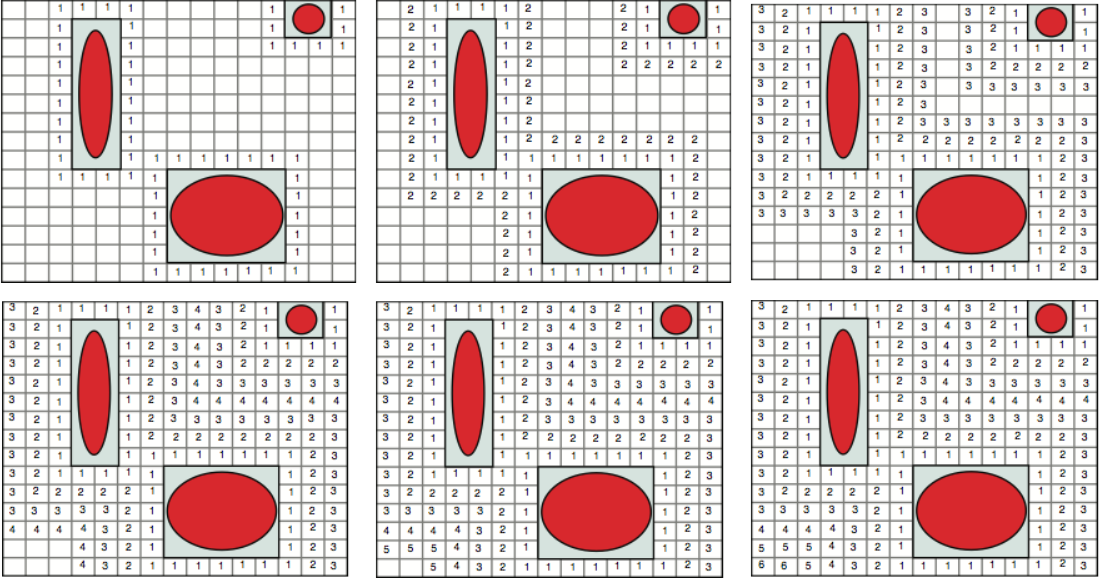
\includegraphics[width=\textwidth]{./images/chapter5/brushfire0.png}
    \caption{Παράδειγμα Brushfire}
    Πηγή: \href{http://roboscience.org/book/html/Planning/Brushfire.html}{http://roboscience.org/book/html/Planning/Brushfire.html}
    \label{fig:brushfire_example}
\end{figure}



\begin{algorithm}[!htb]
\caption{Obstacle Brushfire}
\label{alg:obstacle_brushfire}
\begin{algorithmic}[1]
    \Function{obstacleBrushfire}{ogm}
        \State $brushfire = np.zeros(ogm.shape)$
        \State $brushfire[ogm > 49] = 1$
        \State $brushfire[ogm == -1] = -1$
        \State $step = 1$
        \State $changed = 1$
        \While{$changed == 1$}
            \State $changed = 0$
            \For{$i$ = 1 to ($brushfire.width$ - 1)}
                \For{$j$ = 1 to ($brushfire.height$ - 1)}
                    \If{$brushfire[i][j] == 0$ and a neighbor's brushfire value is equal to step}
                        \State $brushfire[i][j] = step + 1$
                        \State $changed = 1$
                    \EndIf
                \EndFor
            \EndFor
            \State $step += 1$
        \EndWhile
        \State \Return $brushfire$
            
\end{algorithmic}
\end{algorithm}

Ο brushfire εμποδίων παρουσιάζεται στο \ref{alg:obstacle_brushfire}. Στις γραμμές 2-4 το πεδίο brushfire ορίζεται έτσι ώστε να έχει τις ίδιες διαστάσεις με το ogm, αρχικά με μηδενικές τιμές στον ελεύθερο χώρο, 1 στα εμπόδια και -1 στα άγνωστα σημεία. Για όσο συμβαίνει η εξάπλωση εξετάζονται όλα τα σημεία του brushfire. Εαν σε κάποιο ελεύθερο σημείο δεν έχει φτάσει ακόμα το κύμα αλλά έχει φτάσει σε έναν γείτονα του στην προηγούμενη επανάληψη με τιμή $step$, τότε και στο τρέχον σημείο ανανεώνει το brushfire με τιμή $step + 1$. Η διαδικασία επαναλαμβάνεται εως ότου δεν επέλθει καμία ανανέωση στον πίνακα $brushfire$, δηλαδή μέχρι την πλήρη εξάπλωση των τιμών.

\subsubsection{Υπολογισμός GVD}
\label{subsection:gvd_algorithms}
Εξίσου χρήσιμο με το $brushfire$ του χάρτη είναι και το GVD του. Αυτό υπολογίζεται χρησιμοποιώντας τη μέθοδο skeletonize\footnote{\href{https://scikit-image.org/docs/dev/auto_examples/edges/plot_skeleton.html}{https://scikit-image.org/docs/dev/auto\_examples/edges/plot\_skeleton.html}} της βιβλιοθήκης της skimage της Python. Το GVD έχει τις ίδιες διαστάσεις με το αντίστοιχο OGM και οι τελικές του τιμές θα είναι 1 στα σημεία που ανήκουν σ' αυτό και 0 σε όλα τα υπόλοιπα. Στην μέθοδο skeletonize εισάγεται ως δυαδική εικόνα ο ελεύθερος χώρος του OGM. Όπως φαίνεται στην εντολή 3 του αλγορίθμου \ref{alg:gvd} χρησιμοποιούνται ως είσοδο τα σημεία που έχουν τιμή brushfire μεγαλύτερη από 5, δηλαδή όλα τα ελεύθερα σημεία εκτός από αυτά που είναι πάρα πολύ κοντά στα εμπόδια. Ο OGM πολλές φορές περιέχει ατέλειες πολύ κοντά στα εμπόδια λόγω αστοχίας της διαδικασίας του SLAM. Χαρακτηριστικό παράδειγμα είναι η περίπτωση να θεωρεί ως ελεύθερο χώρο σημεία πίσω από τον τοίχο, εκτός του χώρου, που κανονικά θα έπρεπε να θεωρούνται άγνωστα. Προκειμένου να μην επηρεάσουν τη διαδικασία υπολογισμού του GVD, λαμβάνονται υπόψη τα σημεία που έχουν μια στοιχειώδη απόσταση από τα εμπόδια.


\begin{algorithm}[!ht]
\caption{GVD}
\label{alg:gvd}
\begin{algorithmic}[1]
    \Function{gvd}{brushfire}
        \State $voronoi = np.zeros(brushfire.shape)$
        \State $voronoi[brushfire >= 5] = 1$
        \State $voronoi = skimage.morphology.skeletonize(voronoi)$
        \State \Return $voronoi$
\end{algorithmic}
\end{algorithm}



\subsection{Υπολογισμός τοπολογικού γράφου του χώρου}
\label{subsection:find_topology}

Το GVD ενός χάρτη περιέχει σημαντικές πληροφορίες για το περιβάλλον. Κρύβει μέσα του τόσο τα όρια των δωματίων όσο και την δομή τους. Επομένως, χρειάζεται να εξαχθούν σημεία που περιέχουν αυτές τις πληροφορίες. Πιο σημαντικοί είναι οι κόμβοι που αντιστοιχούν στις πόρτες του χώρου, καθώς με αυτούς μπορεί να διαχωριστεί αποτελεσματικά ο χάρτης στα δωμάτια του. Η μέθοδος βασίστηκε σε μια αντίστοιχη μελέτη γνωστού χώρου που είχε πραγματοποιηθεί στο \cite{sikoudi}. 

Η διαδικασία που υλοποιήθηκε αναλύεται στη συνέχεια. Καταρχάς, κάθε σημείο του GVD μπορεί να έχει από ένα έως τέσσερα γειτονικά σημεία τα οποία ανήκουν και αυτά στο GVD. Ανάλογα μάλιστα με το πλήθος των γειτόνων, μπορούν να εξαχθούν πληροφορίες για το κάθε σημείο. Έτσι, παρατηρώντας και το \autoref{fig:gvd_neighbors_example} τα σημεία με έναν μόνο γείτονα βρίσκονται στις άκρες του GVD, δηλαδή σε περιοχές που πλησιάζουν σε εμπόδια, όπως οι γωνίες των δωματίων και επισημαίνονται με κίτρινους κύκλους. Αντίστοιχα, τα σημεία με τρεις ή τέσσερις γείτονες βρίσκονται σε πιο κεντρικά, όσον αφορά τις αποστάσεις από τα εμπόδια, σημεία ή σε σημεία διακλάδωσης, όπως η περιοχή μπροστά από μια πόρτα, όπου και το διάγραμα διακλαδίζεται και επισημαίνονται με κόκκινους κύκλους. Το σημείο που αντιστοιχεί σε πόρτα επισημαίνεται με πράσινο χρώμα και όπως φαίνεται έχει δύο γείτονες. Όλοι αυτοί οι κόμβοι πρέπει να εξαχθούν από το GVD για να δημιουργηθεί ο τοπολογικός γράφος του χώρου.

Πρώτα, σαρώνεται ο χώρος, ώστε να βρεθούν όλα τα σημεία του GVD με έναν, τρεις ή περισσότερους γείτονες. Αυτά αν και δεν χρειάζονται για την εύρεση των πορτών και τον διαχωρισμό των δωματίων, μπορούν να χρησιμοποιηθούν για άλλους λόγους, όπως παρουσιάζεται στο \ref{section:room_classification}.

Έπειτα, πρέπει να μελετηθούν τα σημεία με δύο γείτονες για να εξαχθούν οι κόμβοι οι οποίοι είναι πιθανό να αποτελούν πόρτες στον χώρο. Για την επίτευξη αυτού θα χρησιμοποιηθεί η τιμή brushfire που έχουν αυτά τα σημεία. Συγκεκριμένα, τα σημεία πόρτες παρουσιάζουν τοπικό ακρότατο στην τιμή brushfire τους. Αυτό γίνεται εύκολα αντιληπτό εαν σκεφτεί κανείς πως για να περάσει το ρομποτικό όχημα, αλλά και ένας άνθρωπος, από μια πόρτα θα πλησιάσει τα εμπόδια, θα φτάσει σε μια ελάχιστη απόσταση ακριβώς στην ευθεία της πόρτας και μετά θα αρχίσει να απομακρύνεται από αυτά. Η ιδιότητα αυτή είναι καθοριστική, καθώς οι υποψήφιες πόρτες μπορούν να βρεθούν, εαν υπολογιστούν τα τοπικά ελάχιστα του brushfire στα σημεία που ανήκουν στο GVD και έχουν δύο γείτονες. Αυτό φαίνεται και στο \autoref{fig:brushfire_minimum_example} όπου έχουν επισημανθεί τα σημεία που ανήκουν στο GVD, ενώ για κάθε σημείο έχει γραφεί το brushfire του. Πράγματι τα σημεία με πράσινο αποτελούν το τοπικό ελάχιστο του brushfire πάνω στο GVD. 

Η διαδικασία που υλοποιήθηκε ελέγχει για κάθε σημείο του GVD με δύο γείτονες εαν έχει την ελάχιστη brushfire τιμή σε μια περιοχή 20x20 γύρω απ' αυτό, συγκρίνοντας μόνο σημειά που ανήκουν στο διάγραμμα Voronoi. Έτσι, βρίσκονται τα τοπικά ελάχιστα τα οποία, όμως, χρειάζονται περαιτέρω επεξεργασία. Όπως φαίνειται και στο \ref{fig:brushfire_minimum_example} για κάθε πόρτα περισσότερα από ένα σημεία αποτελούν τοπικό ελάχιστο, καθώς ο αλγόριθμος brushfire εξαπλώνεται και στα οχτώ γειτονικά του σημεία. Για την αναγωγή κάθε τοπικού ελαχίστου στο πιο αντιπροσωπευτικό της πόρτας, ομαδοποιούνται τα σημεία ανά γειτονιές και κρατιέται το μεσαίο από κάθε ομάδα ως υποψήφιος κόμβος πόρτας.

\begin{figure}[!htb]
    \centering
    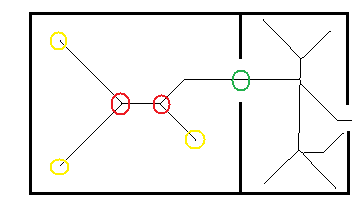
\includegraphics[width=0.5\textwidth]{./images/chapter5/rooms_3_gvd_1_3_neighbors_pinned.png}
    \caption{Κόμβοι τοπολογικού γράφου}
    \label{fig:gvd_neighbors_example}
\end{figure}


\begin{figure}[!htb]
    \centering
    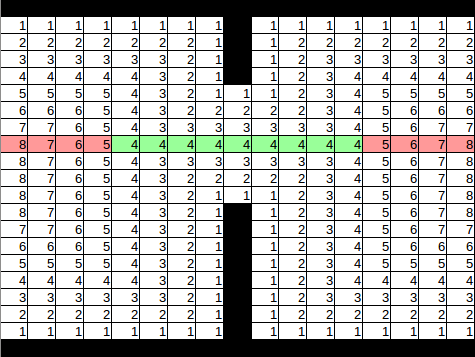
\includegraphics[width=0.5\textwidth]{./images/chapter5/brushfire_gvd_example.png}
    \caption{Τοπικό Ελάχιστο Brushfire στις πόρτες}
    \label{fig:brushfire_minimum_example}
\end{figure}


Η διαδικασία παρουσιάζεται στον αλγόριθμο \ref{alg:topological_nodes} και χρησιμοποιεί τα ήδη υπολογισμένα πεδία brushfire και GVD του χώρου. Στις εντολές 2-14 γίνεται η πρώτη εξαγωγή χρήσιμων κόμβων από το GVD. Στη συνέχεια στις εντολές 16-26 ομαδοποιούνται οι κόμβοι με δύο γείτονες που βρίσκονται στην ίδια γειτονιά, δηλαδή που αντιστοιχούν στην ίδια πόρτα, και κρατιέται ο μεσαίος κόμβος ως υποψήφιος κόμβος πόρτας.



\begin{algorithm}[!htb]
\caption{Topological Nodes}
\label{alg:topological_nodes}
\begin{algorithmic}[1]
    \Function{topologicalNodes}{brushfire, gvd}
        \State $nodes = []$
        \For{every point $(x,y)$ of gvd, where $gvd == 1$}
            \State count gvd neighbors of point $(x,y)$
            \If{number of neighbors is 1, 3 or 4}
                \State $nodes.append((x,y))$
            \EndIf
            \If{number of neighbors is 2}
                \State Check if $brushfire[x,y]$ is minimum in a 20x20 area
                \If{ $brushfire[x,y]$ is min }
                    \State $nodes.append((x,y))$
                \EndIf
            \EndIf
        \EndFor
        \State \Comment{Recheck nodes with 2 neighbors to keep one point of each neighborhood}
        \State $final\_nodes = []$
        \State add all nodes that don't have 2 neighbors to $final\_nodes$
        \State Group nodes with 2 neighbors to lists of points of same line
        \For{each list of points}
            \If{number of nodes in list is odd}
                \State add middle point to $final\_nodes$
            \Else
                \State add first of the two middle points to $final\_nodes$
            \EndIf
        \EndFor
        \State \Return $final\_nodes$
\end{algorithmic}
\end{algorithm}

Τα ενδιάμεσα αποτελέσματα παρουσιάζονται και στα επόμενα σχήματα. Συγκεκριμένα, οι μικρές ευθείες των τοπικών ελαχίστων παρουσιάζονται στο \ref{fig:rooms_3_door_lines}, όπου με μπλε σημειώνονται τα σημεία που πράγματι είναι κοντά σε μια πόρτα και με πράσινο σημεία που ενώ είναι ακρότατα του χάρτη, δεν αντιστοιχούν σε κάποια πόρτα. Μάλιστα, αυτά τα σημεία αποτελούν τοπικά μέγιστα του χώρου. Στην πράξη, λοιπόν, αν και ο αλγόριθμος αναζητάει τοπικά ελάχιστα μόνο, είναι πολύ πιθανό να βρει και τοπικά μέγιστα, καθώς για κάθε σημείο του GVD η brushfire τιμή του συγκρίνεται με τις γύρω 20x20 τιμές. Αυτό σημαίνει ότι σε περιπτώσεις που παρουσιάζονται και τοπικά μέγιστα, εαν αυτά αποτελούνται από περισσότερα από 20 σειριακά σημεία, θα κρατηθούν ορισμένα από αυτά. Για να καταλάβει ο αλγόριθμος ότι πρόκειται πράγματι για μέγιστο και όχι ελάχιστο θα χρειαζόταν να ελέγξει μια μεγαλύτερη περιοχή από τα 20x20 σημεία που καλύπτει ήδη, κάτι που όμως δεν θα έλυνε αποτελεσματικά το πρόβλημα για κάθε χώρο. Πάντα θα υπάρχει ένα περιβάλλον που θα χρειάζεται μεγαλύτερο πεδίο σύγκρισης των τιμών brushfire με το τρέχον σημείο. Το πρόβλημα διαχωρισμού των πραγματικών πορτών, λοιπόν, θα αντιμετωπιστεί στην επόμενη υποενότητα με μια διαφορετική διαδικασία.

Στο \autoref{fig:rooms_3_doors} παρουσιάζονται τα αντιπροσωπευτικά σημεία κάθε μικρού ευθύγραμμου τμήματος του προηγούμενου σχήματος με τα αντίστοιχα χρώματα. Οι κόμβοι αυτοί αποτελούν το σύνολο των υποψήφιων κόμβων πόρτας του χώρου. 

Τέλος, στο \autoref{fig:rooms_3_nodes_with_doors} παρουσιάζονται όλοι οι κόμβοι που επιστρέφει ο αλγόριθμος \ref{alg:topological_nodes}. Με μπλε εμφανίζονται οι τελικές πόρτες και με κόκκινο όλα τα υπόλοιπα σημεία στα εσωτερικά των δωματίων.


\begin{figure}{\textwidth} 
    \centering
    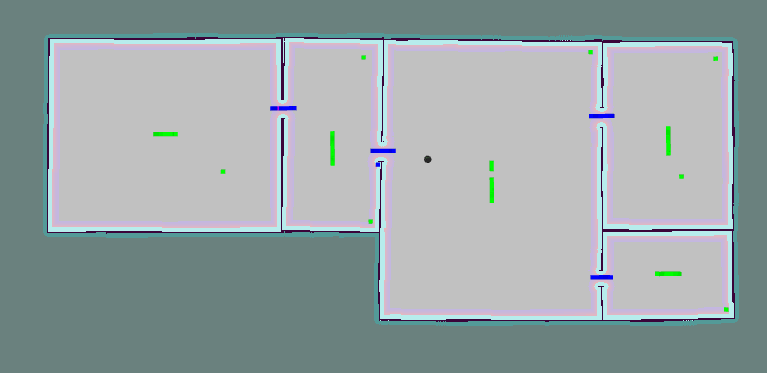
\includegraphics[width=0.7\textwidth]{./images/chapter5/rooms_3_door_lines.png}
    \caption{Ευθείες με Κόμβους Τοπικών Ακροτάτων}
    \label{fig:rooms_3_door_lines}
\end{figure}
\begin{figure}{\textwidth} 
    \centering
    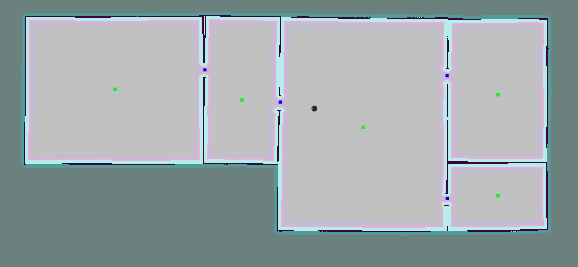
\includegraphics[width=0.7\textwidth]{./images/chapter5/rooms_3_doors.png}
    \caption{Υποψήφιοι Κόμβοι Πόρτες}
    \label{fig:rooms_3_doors}
\end{figure}
\begin{figure}{\textwidth} 
    \centering
    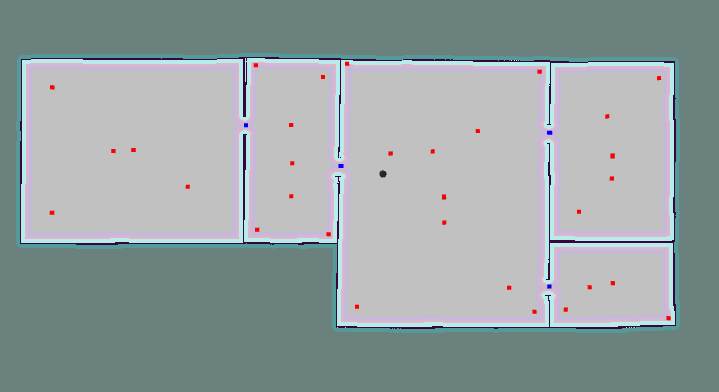
\includegraphics[width=0.7\textwidth]{./images/chapter5/rooms_3_nodes_with_doors.png}
    \caption{Τελικοί Κόμβοι Τοπολογικού Γράφου του Χώρου}
    \label{fig:rooms_3_nodes_with_doors}
\end{figure}


\subsection{Ορισμός των Κόμβων Πόρτας}
\label{subsection:find_door_nodes}

Το επόμενο βήμα της διαδικασίας είναι η εύρεση των πραγματικών πορτών του χώρου. Ως πιθανοί κόμβοι πόρτας λαμβάνονται όλοι οι κόμβοι της προηγούμενης διαδικασίας που έχουν δύο ακριβώς γείτονες στο GVD. Όπως αναλύθηκε νωρίτερα, υπάρχουν περισσότεροι υποψήφιοι κόμβοι από τις πραγματικές πόρτες ακόμη και σε περιβάλλοντα με απλή εσωτερική δομή. Φυσικά, όσο περισσότερα εμπόδια περιέχει ο χώρος, τόσα περισσότερα πιθανά σημεία πόρτας υπάρχουν. 

Η εύρεση των πραγματικών πορτών από το σύνολο των υποψήφιων βασίζεται σε μια σημαντική ιδιότητα κάθε πόρτας. Οι κόμβοι των πραγματικών πορτών βρίσκονται ενδιάμεσα δύο εμποδίων, των δύο τοιχών της πόρτας. Τα δύο αυτά σημεία σχηματίζουν, μάλιστα, μια ευθεία στον χώρο στην προέκταση της οποίας υπάρχει σημαντικό ποσοστό κατειλλημένου χώρου από την προέκταση των εμποδίων. Στόχος είναι να βρεθεί ένα κατάλληλο κατώφλι προσαρμοσμένο στον κάθε χάρτη, ώστε να συγκριθούν τα ποσοστά όλων των κόμβων με αυτό και να επιλεγούν μόνο αυτοί που έχουν μεγαλύτερο ποσοστό από το όριο αυτό.

Στο \autoref{fig:door_line_example} παρουσιάζονται τρεις διαφορετικές περιπτώσεις κόμβων που είναι υποψήφιοι να είναι κόμβοι πόρτες. Οι κόμβοι αυτοί έχουν κόκκινο χρώμα, ενώ τα σημεία που αποτελούν τα πιο κοντινά εμπόδια έχουν μπλε χρώμα. Η ευθεία των εμποδίων εμφανίζεται με διακεκομμένη πράσινη γραμμή. Στο πρώτο σχήμα, ο υποψήφιος κόμβος πόρτας βρίσκεται κοντά σε μια γωνία του δωματίου. Δεν αποτελεί σημείο πόρτας διότι δεν βρίσκεται ανάμεσα στα δύο σημεία των εμποδίων, δηλαδή δεν βρίσκεται πάνω στην πράσινη ευθεία. Στο δεύτερο σχήμα, ο υποψήφιος κόμβος αποτελεί σημείο της ευθείας αυτής. Όμως, τα σημεία που ανήκουν στην ευθεία κατά κύριο λόγο αποτελούν ελεύθερα σημεία του χώρου, πράγμα που σημαίνει ότι δεν υπάρχουν οι αναμενόμενοι τοίχοι στην προέκταση των εμποδίων. Τέλος, στο τρίτο σχήμα παρουσιάζεται η περίπτωση της πραγματικής πόρτας. Είναι εύκολα διακριτό το γεγονός ότι μεγάλο ποσοστό των σημείων που ανήκουν στην εν λόγω ευθεία είναι σημεία εμποδίων.


\begin{figure}[!htb]
    \centering
    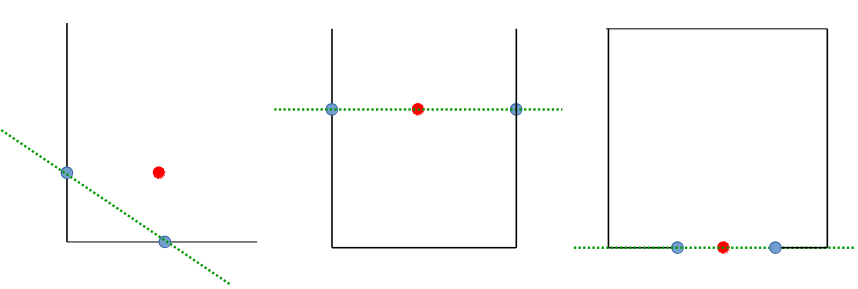
\includegraphics[width=0.9\textwidth]{./images/chapter5/door_line_example.png}
    \caption{Παραδείγματα Ελέγχου Κόμβων Πόρτας}
    \label{fig:door_line_example}
\end{figure}



\medskip
Ο αλγόριθμος παρουσιάζεται σε αναλυτική μορφή στο \ref{alg:find_door_nodes}. Η διαδικασία συνοψίζεται για κάθε υποψήφιο κόμβο στα παρακάτω βήματα:
\begin{itemize}
    \setlength\itemsep{-0.2em}
    \item Εύρεση κοντινότερων εμποδίων του κόμβου
    \item Έλεγχος πλήθους αυτών των σημείων
    \item Εύρεση της ευθείας των σημείων αυτών και έλεγχος της εγγύτητας του κόμβου με αυτήν
    \item Μέτρηση ποσοστού κάλυψης στο OGM σε ένα πεπερασμένο μήκος της ευθείας αυτής
    \item Υπολογισμός κατωφλιού απόφασης
    \item Σύγκριση ποσοστού με κατώφλι αποδοχής κόμβου ως πόρτα
\end{itemize}


Το πρώτο βήμα κάνει χρήση της συνάρτησης \ref{alg:closestObstacleBrushfire} η οποία δέχεται ως είσοδο ένα OGM και τον τρέχοντα κόμβο και εκτελεί brushfire με αρχή το σημείο αυτό, μέχρι να φτάσει η εξάπλωση στο πρώτο εμπόδιο. Τότε, η διαδικασία εκτελείται για άλλη μια επανάληψη και στη συνέχεια τερματίζεται. Η ύπαρξη της μιας παραπάνω φοράς είναι αναγκαία, καθώς σε περίπτωση που σε μια πόρτα μεσολαβεί άρτιος αριθμός ελεύθερων σημείων, ο κόμβος της πόρτας θα βρίσκεται στην μια πλευρά πιο κοντά κατά ένα pixel. Με τον τρόπο αυτό, όμως, θα εντοπιστούν και οι δύο πλευρές των εμποδίων. Στη συνέχεια, τα εμπόδια όπου έφτασε ο brushfire ομαδοποιούνται σε γειτονικά και επιλέγεται να επιστραφεί από κάθε ομάδα το σημείο που είναι πιο κοντά στον κόμβο εκκίνησης. Η εντολή αυτή καλείται στην γραμμή 4. 

Έπειτα, πραγματοποιείται ο έλεγχος του πλήθους των σημείων των εμποδίων στην γραμμή 5. Το επόμενο βήμα υλοποιείται με τις εντολές 7-11. Μετά μετράται το ποσοστό κάλυψης των σημείων της ευθείας. Πολλές φορές όμως ένα OGM μπορεί να περιέχει ατέλειες. Γι αυτό τον λόγο ο αλγόριθμος χρησιμοποιεί σημεία που είναι γύρω από την ευθεία. Συγκεκριμένα, χρησιμοποιείται το ευθύγραμμο τμήμα των δύο σημείων των εμποδίων της εντολής 4 με 50 pixels επέκταση προς κάθε πλευρά. Επίσης, το πλάτος της ευθείας από 1 pixel αυξάνεται στα 5 pixel. Με τον τρόπο αυτό εξασφαλίζεται ότι οι γύρω τοίχοι θα βρίσκονται μέσα στην περιοχή που προσμετράται στο ποσοστό κάλυψης. Άλλωστε το πάχος των τοιχών στα συνήθη OGM είναι μεγαλύτερο του ενός pixel, συνεπώς οι επεκτάσεις θα οδηγήσουν σε ακόμα μεγαλύτερο ποσοστό κατάλληψης.

Το πιο σημαντικό βήμα της διαδικασίας αυτής είναι η επιλογή ενός σωστού κατωφλιού, ανάλογου του κάθε χάρτη. Θα ήταν λάθος η χρήση ενός σταθερού αριθμού, καθώς χάνεται η δυνατότητα γενίκευσης της διαδικασίας σε κάθε νέο χάρτη. Μελετήθηκαν οι τιμές των ποσοστών πορτών από διάφορους πολύπλοκους χώρους και προέκυψαν τα εξής δύο συμπεράσματα:
\begin{itemize}
    \setlength\itemsep{-0.2em}
    \item Όλοι οι κόμβοι που δεν αποτελούν πόρτες έχουν ποσοστό μικρότερο από 20\%.
    \item Οι κόμβοι που είναι πόρτες έχουν σημαντικά πολύ μεγαλύτερη τιμή της μετρικής αυτής.
\end{itemize}
Η διαφορά των τιμών είναι τόσο μεγάλη σε κάθε περίπτωση που το τελικό όριο μπορεί να βρεθεί εντοπίζοντας την μεγαλύτερη πρώτη διαφορά των ταξινομημένων τιμών. Για παράδειγμα, στην επόμενη λίστα παρουσιάζονται οι τιμές από το σχήμα \ref{fig:rooms_3_doors}: 


$[0.01126761$, $0.01344538$, $0.01587302$, $0.12833333$, $0.19310345$, $0.24833333$, $0.49579832]$

\smallskip

Οι πρώτες τρεις τιμές που είναι κοντά στο 1\% αφορούν σημεία που δεν αντιστοιχούν σε πόρτες. Αντίθετα, οι υπόλοιπες τέσσερις είναι από κόμβους πόρτας. Φαίνεται ότι ενώ οι μεν τιμές κυμαίνονται κοντά στο 1\%, οι δε είναι αρκετά πάνω από το 10\% με την μεγαλύτερη σχεδόν στο 50\%. Επομένως, είναι αρκετά διακριτό το όριο σε κάθε χάρτη και εντοπίζεται στην μεγαλύτερη τιμή των πρώτων διαφορών των τιμών, για την οποία το όριο θα είναι μικρότερο του 20\%. Στόχος είναι να τεθεί ως κατώφλι το μεγαλύτερο ποσοστό κάλυψης από τους κόμβους που δεν αποτελούν πόρτες. Έτσι, καθώς οι πραγματικές πόρτες θα έχουν μεγαλύτερο ποσοστό, θα επιστρέφονται ορθά από τον αλγόριθμο. Τέλος, σημειώνεται ότι προστίθεται και μια μηδενική τιμή στην λίστα, ώστε σε περίπτωση που όλοι οι κόμβοι αποτελούν πόρτες, να μπορεί να τεθεί το όριο στο μηδέν και να φέρει ο αλγόριθμος τα σωστά αποτελέσματα.

Το τελευταίο βήμα είναι η σύγκριση κάθε τιμής με το κατώφλι που υπολογίστηκε και η τελική απόφαση των κόμβων πόρτας κάθε χώρου.

Να σημειωθεί ότι η διαδικασία αυτή θεωρεί την ύπαρξη έστω μίας πόρτας στον χάρτη. Σε περίπτωση που δεν υπάρχει, θα θεωρήσει ως πόρτα το σημείο που προσεγγίζει με μεγαλύτερη ακρίβεια τα χαρακτηριστικά των πορτών που σχολιάστηκαν νωρίτερα.



\begin{algorithm}[H]
\caption{Closest Obstacle Brushfire}
\label{alg:closestObstacleBrushfire}
\begin{algorithmic}[1]
    \Function{closestObstacleBrushfire}{start, ogm}
        \State $brushfire = np.zeros(ogm.shape)$
        \State $brushfire[ogm > 49] = 1$
        \State $brushfire[ogm == -1] = -1$
        \State $brushfire[start] = 2$
        \State $final\_obstacles = []$
        \State $step = 2$
        \State $changed = 1$
        \State $last = 1$
        \State $found = 0$
        \While{$changed == 1$ and $last == 0$}
            \State $changed = 0$
            \If{$found == 1$}
                \State $last = 1$
            \EndIf
            \For{$i$ = 1 to (brush.width - 1)}
                \For{$j$ = 1 to (brush.height - 1)}
                    \If{$brushfire[i][j] == 0$ and a neighbor's brushfire value is equal to step}
                        \State $brushfire[i][j] = step + 1$
                        \State $changed = 1$
                    \ElsIf{$brushfire[i][j] == 1$ and a neighbor's brushfire value is equal to step}
                        \State $brushfire[i][j] = -2$
                        \State $found = 1$
                    \EndIf
                \EndFor
            \EndFor
            \State $step += 1$
        \EndWhile
        \State Set $obstacles$ equal to indexes where $brushfire[][] == -2$
        \State Group $obstacles$ to neighborhoods
        \For{each neighborhood}
            \State Compute closest obstacle $ob$ to $start$
            \State $final\_obstacles.append(ob)$
        \EndFor
        \State \Return $final\_obstacles$
            
\end{algorithmic}
\end{algorithm}




\begin{algorithm}[H]
\caption{Find Door Nodes}
\label{alg:find_door_nodes}
\begin{algorithmic}[1]
    \Function{findDoorNodes}{$nodes, ogm, gvd$}
        \State $doorNodes = [], candidateDoors = [], perc = []$
        \For{each $node$ in $nodes$}
            \State $ob = closestObstacleBrushfire(node, ogm)$
            \If{$length(ob) == 2$}
                \State $candidateDoors.append(node)$
                \State find $line$ of 2 obstacles $ob$
                \State \Comment{Door nodes should be inside obstacles' line}
                \If{$node$'s distance from line is larger than 5}
                    \State Continue
                \EndIf
                \State Collect indexes of points of $line$ extended by 50 pixels at each direction outside the $ob$ line segment and with 5 pixel width
                \State Compute occupancy percentage of extended line
                \State Append percentage to $perc$
            \EndIf
        \EndFor
        \Comment{Compute right threshold}
        \State $perc.append(0.0)$
        \If{$length(perc) > 1$}
            \State $perc\_copy = numpy.array(perc).sort()$
            \State $diff = numpy.diff(perc\_copy)$
            \State $max\_value = max(diff), max\_index = diff.argmax()$
            \State $threshold = perc\_copy[max\_index]$
            \While{$threshold > 0.20$}
                \State $max = 0, current\_index = -1$
                \For{$i$ in $range(len(diff))$}
                    \If{$diff[i] > max$ and $diff[i]$ not in $max\_values$}
                        \State $max = diff[i], current\_index = i$
                    \EndIf
                \EndFor
            \State $max\_values.append(max)$
            \State $threshold = perc\_copy[current\_index]$
            \EndWhile
        \ElsIf{$length(perc) == 1$}
            \State $threshold = perc[0] - 0.001$
        \Else
            \State \Return $None$
        \EndIf
        \For{each $node$ in $candidateDoors$}
            \If{$perc$ of $node > threshold$}
                \State $doorNodes.append(node)$
            \EndIf
        \EndFor
        \State \Return $doorNodes$
\end{algorithmic}
\end{algorithm}


\subsection{Διαχωρισμός Κόμβων σε Δωμάτια}
\label{subsection:find_room_nodes}

Το τελευταίο μέρος της μελέτης του χώρου αποτελείται από διαχωρισμό του συνόλου των κόμβων του χάρτη στα επιμέρους δωμάτια στα οποία ανήκουν. Ο \autoref{alg:find_rooms} δέχεται ως είσοδο το GVD και το OGM του χώρου, το σύνολο των κόμβων και τους κόμβους πόρτες και επιστρέφει δύο λίστες, την $rooms$ που περιέχεί τους κόμβους διαχωρισμένους σε επιμέρους λίστες άνα δωμάτιο και την $roomDoors$ που περιέχει επιμέρους λίστες των πορτών κάθε δωματίου. Κατά την υλοποίηση του αλγορίθμου δημιουργήθηκε ένας ακόμη αλγόριθμος που στοχεύει στην εύρεση των γειτονικών κόμβων ενός κόμβου εκτελώντας brushfire πάνω στο GVD από τον αρχικό κόμβο μέχρι τους επόμενους γειτονικούς. Δημιουργήθηκαν, μάλιστα, δύο παραλλαγές, οι \ref{alg:gvdNeighborBrushfire} και \ref{alg:gvdNeighborSplitBrushfire} προκειμένου να διαχωρίζονται οι γείτονες των κόμβων πόρτας σε δύο διαφορετικές λίστες στην δεύτερη περίπτωση αντί για μία, για την ευκολότερη διαχείρηση των δεδομένων. 

Ο αλγόριθμος διαχωρισμού δωματίων \ref{alg:find_rooms} εκκινεί από κάθε πόρτα του χώρου και αναζητά γειτονικούς κόμβους κινούμενος πάνω στο GVD και τους κατατάσσει στα αντίστοιχα δωμάτια. Η διαδικασία πραγματοποιείται για κάθε πλευρά της πόρτας, δηλαδή για κάθε δωμάτιο και επαναληπτικά για όλες τις πόρτες του χάρτη, ώστε να καλυφθούν όλοι κόμβοι των επιμέρους χώρων. Ο αλγόριθμος αυτός είναι χρήσιμος και στην ταξινόμηση του κάθε χώρου σε δωμάτιο ή διάδρομο, όπως μελετήθηκε στο \ref{section:room_classification}.


\begin{algorithm}[!htb]
\caption{Gvd Neighbor Brushfire}
\label{alg:gvdNeighborBrushfire}
\begin{algorithmic}[1]
    \Function{gvdNeighborBrushfire}{start, nodes, gvd}
        \State $brushfire = np.zeros(gvd.shape)$
        \State $brushfire[gvd == 1] = 1$
        \State $brushfire[nodes] = -1$
        \State $brushfire[start] = 2$
        \State $step = 2$, $changed = 1$
        \While{$changed == 1$}
            \State $changed = 0$
            \For{$i$ = 1 to ($brushfire.width$ - 1)}
                \For{$j$ = 1 to ($brushfire.height$ - 1)}
                    \If{$brushfire[i][j] == 1$ and a neighbor's brushfire value is equal to step}
                        \State $brushfire[i][j] = step + 1$, $changed = 1$
                    \ElsIf{$brushfire[i][j] == -1$ and a neighbor's brushfire value is equal to step}
                        \State $brushfire[i][j] = -2$
                    \EndIf
                \EndFor
            \EndFor
            \State $step += 1$
        \EndWhile
        \State Set $ind$ equal to indexes where $brushfire[][] == -2$   
        \State \Return $ind$
\end{algorithmic}
\end{algorithm}


\begin{algorithm}[H]
\caption{Gvd Neighbor Split Brushfire}
\label{alg:gvdNeighborSplitBrushfire}
\begin{algorithmic}[1]
    \Function{gvdNeighborSplitBrushfire}{start, nodes, gvd}
        \State $brushfire = np.zeros(gvd.shape)$
        \State $brushfire[gvd == 1] = 1$
        \State $brushfire[nodes] = -1$
        \State $brushfire[start] = 2$
        \State Compute 2 gvd neighbors $nn$ of $start$ point
        \State $brushfire[nn[0]] = 3$
        \State $step = 3$, $changed = 1$
        \While{$changed == 1$}
            \State $changed = 0$
            \For{$i$ = 1 to ($brushfire.width$ - 1)}
                \For{$j$ = 1 to ($brushfire.height$ - 1)}
                    \If{$brushfire[i][j] == 1$ and a neighbor's brushfire value is equal to step}
                        \State $brushfire[i][j] = step + 1$, $changed = 1$
                    \ElsIf{$brushfire[i][j] == -1$ and a neighbor's brushfire value is equal to step}
                        \State $brushfire[i][j] = -2$
                    \EndIf
                \EndFor
            \EndFor
            \State $step += 1$
        \EndWhile
        \State Set $ind[0]$ equal to indexes where $brushfire[][] == -2$
        
        \State $brushfire[nn[1]] = 3$
        \State $step = 3$, $changed = 1$
        \While{$changed == 1$}
            \State $changed = 0$
            \For{$i$ = 1 to ($brushfire.width$ - 1)}
                \For{$j$ = 1 to ($brushfire.height$ - 1)}
                    \If{$brushfire[i][j] == 1$ and a neighbor's brushfire value is equal to step}
                        \State $brushfire[i][j] = step + 1$, $changed = 1$
                    \ElsIf{$brushfire[i][j] == -1$ and a neighbor's brushfire value is equal to step}
                        \State $brushfire[i][j] = -2$
                    \EndIf
                \EndFor
            \EndFor
            \State $step += 1$
        \EndWhile
        \State Set $ind[1]$ equal to indexes where $brushfire[][] == -2$
        \State \Return $ind$
\end{algorithmic}
\end{algorithm}



\begin{algorithm}[!htb]
\caption{Find Rooms}
\label{alg:find_rooms}
\begin{algorithmic}[1]
    \Function{findRooms}{$gvd, doors, nodes, ogm$}
        \State $rooms = []$, $roomDoors = []$, $visited = []$
        \For{each $door$ in $doors$}
            \State $visited.append(door)$
            \State $nn = gvdNeighborSplitBrushfire(door, nodes, gvd)$
            \State Discard nodes of $nn$ that are in $visited$
            \For{$i$ in $range(2)$}
                \State $current\_room = [], next = []$
                \If{$length(nn[i]) == 0$}
                    \State Continue
                \EndIf
                \State $current\_room.append(nn[i][0])$ \Comment{Start from first node}
                \State $next = nn[i][1:]$ \Comment{Add rest to list for next iteration}
                \State $current = current\_room[:]$, $all\_doors = []$
                \State $all\_doors.append(door)$
                \While{$current != []$}
                    \For{$node$ in $current$}
                        \If{$node$ in $doors$ and $node != door$}
                            \State $all\_doors.append(node)$
                        \ElsIf{$node$ not in $doors$}
                            \State $visited.append(node)$
                            \State $node\_nn = gvdNeighborBrushfire(node, nodes, gvd)$
                            \For{each node $n$ in $node\_nn$}
                                \If{$n$ in $doors$ and $n != door$ and $n$ not in $all\_doors$}
                                    \State $all\_doors.append(n)$
                                \ElsIf{$n$ not in $visited$ and $n$ not in $doors$}
                                    \State $visited.append(n)$
                                    \State $next.append(n)$
                                    \State $current\_room.append(n)$
                                \EndIf
                            \EndFor
                        \EndIf
                    \EndFor
                    \State $current = next$, $next = []$
                \EndWhile
                \State $roomDoors.append(all\_doors)$
                \State $rooms.append(current\_room)$
            \EndFor
        \EndFor  
        \State \Return $rooms, roomDoors$
\end{algorithmic}
\end{algorithm}



\newpage
\section{Πειράματα Ακολουθίας Δωματίων}
\label{sec:experiments_room_sequence}

Στο δέυτερο μέρος των πειραμάτων χρησιμοποιούνται 70 χάρτες από αυτούς που χρησιμοποιήθηκαν και στο πρώτο μέρος των πειραμάτων με σκοπό τη μελέτη του μήκους της διαδρομής επίσκεψης των δωματίων κάθε χώρου. Συγκρίθηκαν 3 διαφορετικοί αλγόριθμοι, οι:

\begin{itemize}
    \setlength\itemsep{-0.2em}
    \item Επιλογή Κοντινότερου Επόμενου Δωματίου (Κοντινότερος Γείτονας)
    \item Anneal Hill Climb
    \item Random Restart Hill Climb
\end{itemize}

Ο πρώτος αποτελεί μια άπληστη μέθοδο επιλογής, όπου κάθε φορά επιλέγεται ο τρέχων καλύτερος επόμενος κόμβος στην ακολουθία, δηλαδή ο κοντινότερος. Είναι μια απλή και γρήγορη αλλά υποβέλτιστη μέθοδος, εφαρομογή ουσιαστικά του αλγορίθμου επιλογής κοντινότερου γείτονα. Οι δύο άλλοι αναπτύχθηκαν στην \autoref{subsection:room_sequence_implementation} και η σύγκριση τους με την άπληστη μέθοδο καταδεικνύει την αποτελεσματικότητα τους. Επίσης, επισημαίνεται ότι οι δύο HC αλγόριθμοι εκτελέστηκαν για πλήθος επαναλήψεων ίσο με 500 φορές επί το πλήθος των πορτών του χάρτη. Σημαντική παρατήρηση είναι ότι ο χρόνος εκτέλεσης και των τριών αλγορίθμων είναι παρόμοιος και αμελητέος.


Ορισμένα τελικά αποτελέσματα μήκους της συνολικής ακολουθίας επίσκεψης των πορτών σε τιμές brushfire, δηλαδή σε μήκος πάνω στο εκάστοτε OGM είναι:


\begin{longtable}{| p{.20\textwidth} | p{.20\textwidth} | p{.20\textwidth} | p{.20\textwidth} |}

    \caption{Επιλεγμένα Αποτελέσματα Μήκους Ακολουθίας Δωματίων}
    \label{tab:room_sequence_results}
    \hline
    \rowcolor[gray]{0.8}
    Κοντινότερος Γείτονας & Anneal HC & RRHC & Ποσοστό Βελτίωσης με RRHC \\ \hline
    $2809$ & $5201$ & $2809$ & $0$\%\\ \hline
    $3338$ & $6870$ & $2979$ & $10.6$\%\\ \hline
    $7928$ & $11990$ & $7698$ & $2.9$\%\\ \hline
    $2414$ & $2766$ & $2318$ & $3.9$\%\\ \hline
    $2769$ & $4087$ & $2519$ & $9.0$\%\\ \hline
    $2834$ & $3766$ & $2834$ & $0$\%\\ \hline
    $11466$ & $13762$ & $10331$ & $9.8$\%\\ \hline
    $996$ & $996$ & $849$ & $14.7$\%\\ \hline
    $558$ & $558$ & $558$ & $0$\%\\ \hline
    $1149$ & $1149$ & $849$ & $26.1$\%\\ 
    \hline
\end{longtable}



Από τα πειράματα προέκυψαν τα παρακάτω ευρήματα. Αρχικά, ο αλγόριθμος anneal HC τις περισσότερες φορές δίνει αποτέλεσμα σημαντικά μεγαλύτερο από το απλό εξαιτίας της στοχαστικότητας του, κάτι που τελικά τον θέτει μη ικανοποιητικό. Μόλις σε 12 χάρτες, στις πιο απλές περιπτώσεις, οι τιμές του anneal HC ήταν ίσες με τις τιμές του κοντινότερου γείτονα. 

Επιπλέον, ο RRHC δίνει σταθερά ίδια ή καλύτερα αποτελέσματα από τον αλγόριθμο κοντινότερου γείτονα, επομένως, αποτελεί μια σημαντική βελτιωμένη διαδικασία. Σε απλές περιπτώσεις ή περιπτώσεις με μικρό αριθμό δωματίων τα αποτελέσματα των δύο αλγορίθμων είναι συνήθως ίσα, ωστόσο όσο αυξάνεται το πλήθος των δωματίων και μια βέλτιστη λύση γίνεται πιο σύνθετη, τόσο σημαντιότερη είναι η διαφορά των αποτελεσμάτων τον δύο αλγορίθμων. Συγκεκριμένα, σε 31 χάρτες παρατηρήθηκε βελτίωση στο μήκος της διαδρομής, ενώ στους υπόλοιπους 39 τα αποτελέσματα ήταν ίσα. Κατά μέσο όρο το ποσοστό βελτίωσης του μήκους της διαδρομής είναι $7.597$\% στους χάρτες που πράγματι παρουσιάζεται βελτίωση και $3.256$\% συνολικά, ενώ τα τρία μεγαλύτερα ποσοστά είναι $26.1$\%, $15.9$\% και $14.7$\%.



Τα συνολικά αποτελέσματα είναι:
\begin{table}[H]
  \begin{center}
    \caption{Μετρήσεις Μήκους Ακολουθίας Δωματίων}
    \label{tab:room_detection}
    \begin{tabular}{ |>{\columncolor[gray]{0.8}} c | c | }
      \hline
      Χάρτες που παρουσίασαν βελίωση & $31\ /\ 70$ \\ \hline
      Μέση Τιμή βελτίωσης & $3.256\%$ \\ \hline
      Τυπική απόκλιση βελτίωσης & $5.166\%$ \\
      \hline
    \end{tabular}
  \end{center}
\end{table}

Συμπερασματικά, ο anneal HC δεν προσφέρει κάποια βελτίωση, ενώ αντίθετα ο RRHC οδηγεί σε ικανοποιητικά αποτελέσματα και από τη στιγμή που δεν επιφέρει χρονική καθυστέρηση συγκριτικά με απλούστερες μεθόδους, όπως του κοντινότερου γείτονα, μπορεί να χρησιμοποιηθεί για τον υπολογισμό της βέλτιστης ακολουθίας δωματίων κάθε χάρτη.

\section{Πλοήγηση Οχήματος και Κάλυψη του Χώρου}
\label{section:navigation_and_coverage}

Σημαντικό μέρος της εργασίας αποτελεί η δημιουργία του συστήματος πλοήγησης του ρομποτικού οχήματος στον χώρο και η συνεχής καταγραφή των περιοχών που καλύπτουν οι κεραίες που φέρει. Τα δύο αυτά συστήματα είναι η βάση όλης της μελέτης της παρούσας εργασίας. Η υλοποίηση τους παρουσιάζεται στη συνέχεια. 


\subsection{Υλοποίηση Πλοήγησης}
\label{section:navigation_implementation}

Η πλοήγηση του ρομποτικού οχήματος στον εικονικό κόσμο επιτυγχάνεται με τη χρήση του Navigation Stack \ref{section:navigation_stack}. Αυτό διευκολύνει σημαντικά τη διαδικασία, καθώς απαιτεί μόνο τις τρεις μεταβλητές του σημείου στόχου, δηλαδή τη θέση και τον προσανατολισμό του. Το stack παράγει την τροχιά που χρειάζεται να ακολουθήσει το όχημα για να βρεθεί στον ζητούμενο στόχο και του δίνει τις κατάλληλες εντολές ταχύτητας. 

Η ανάπτυξη του συστήματος βασίστηκε στο \cite{navStack} και παρουσιάζεται στους επόμενους δύο αλγορίθμους. Ο πρώτος \ref{alg:go_to_goal} διαβάζει τη θέση και τον προσανατολισμό του σημείου στόχου, τον μετασχηματίζει στην κατάλληλη μορφή, δημιουργεί το μήνυμα $goal$ και το στέλνει στο stack περιμένοντας την επιτυχή εκτέλεση του. Ο δεύτερος \ref{alg:navigation} αποτελεί τον βασικό αλγόριθμο της διαδικασίας και υπολογίζει το τρέχον δωμάτιο διαβάζοντας τη θέση του οχήματος στο OGM και για κάθε δωμάτιο σύμφωνα με την αλληλουχία που έχει υπολογιστεί ανακαλεί τα σημεία στόχους του. Κάθε σημείο διαχωρίζεται σε θέση και προσανατολισμό και καλείται η συνάρτηση \emph{goToGoal}. Τέλος, μόλις το όχημα προσεγγίσει τον στόχο παραμένει εκεί για 0.1 δευτερόλεπτα, για την καλύτερη κάλυψη του χώρου, πριν συνεχίσει για το επόμενο σημείο.


\begin{algorithm}[H]
\caption{Go To Goal}
\label{alg:go_to_goal}
\begin{algorithmic}[1]
    \Function{goToGoal}{target, yaw}
        \State Set $resolution$ equal to map's resolution
        \State Set $origin$ equal to map's origin
        \State $move\_base\_client.wait\_for\_server()$
        \State $goal = MoveBaseGoal()$
        \State $goal.target\_pose.header.frame\_id = 'map'$
        \State $goal.target\_pose.header.stamp = rospy.Time.now()$
        \State $goal.target\_pose.pose.position.x = target[0]*resolution + origin['x']$
        \State $goal.target\_pose.pose.position.y = target[1]*resolution + origin['y']$
        \State $quaternion = tf.transformations.quaternion\_from\_euler(0, 0, yaw)$
        \State $goal.target\_pose.pose.orientation.x = quaternion[0]$
        \State $goal.target\_pose.pose.orientation.y = quaternion[1]$
        \State $goal.target\_pose.pose.orientation.z = quaternion[2]$
        \State $goal.target\_pose.pose.orientation.w = quaternion[3]$
        \State $move\_base\_client.send\_goal(goal)$
        \State $wait = move\_base\_client.wait\_for\_result()$
        \State \Return $move\_base\_client.get\_result()$
\end{algorithmic}
\end{algorithm}



\begin{algorithm}[H]
\caption{Navigation}
\label{alg:navigation}
\begin{algorithmic}[1]
    \Function{navigation}{sequence, rooms}
    \State Read robot's current pose
    \State Compute current room
    \For{each $room$ in $sequence$ starting from current}
        \For{each $pose$ in $room$}
            \State $result = goToGoal(pose['position'], pose['yaw'])$
            \State $rospy.sleep(0.1)$
        \EndFor
    \EndFor
    \State \Return 
\end{algorithmic}
\end{algorithm}

\subsection{Υλοποίηση Κάλυψης Χώρου}
\label{section:coverage_implementation}

Η δεύτερη υλοποίηση αφορά την συνεχή καταγραφή της κάλυψης του χώρου. Το σύστημα αυτό λειτουργεί παράλληλα με όλα τα υπόλοιπα χωρίς να τα επηρεάζει ως μια ξεχωριστή διεργασία. 

Το όχημα φέρει ένα σύνολο αισθητήρων με χαρακτηριστικά τα οποία ορίζονται στην αρχή της διαδικασίας και είναι το μήκος της ακτίνας κάλυψης, το γωνιακό εύρος κάλυψης FOV και η γωνία τοποθέτησης της κεραίας ως προς το εμπρός μέρος του οχήματος. Το σχήμα του πεδίου κάλυψης είναι ουσιαστικά ένα τμήμα ενός κύκλου, όπως φαίνεται και στις δύο εικόνες \ref{fig:sensor_field_example}, όπου με μπλε χρώμα είναι σκιασμένες οι περιοχές κάλυψης. Στην πρώτη το όχημα φέρει μια κεραία με ευρεία γωνία κάλυψης ενώ στην δεύτερη φέρει δύο, μικρότερου εύρους, τοποθετημένες συμμετρικά στις δύο πλευρές του.

\begin{figure}[!htb]
    \centering
    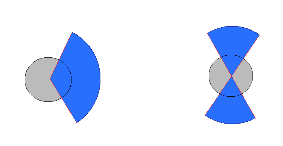
\includegraphics[width=0.4\textwidth]{./images/chapter5/sensor_field_example.png}
    \caption{Παράδειγμα Κάλυψης Αισθητήρων}
    \label{fig:sensor_field_example}
\end{figure}

Στην διπλωματική αυτή εργασία γίνεται μελέτη τριών διαφορετικών στοιχείων της κάλυψης του χώρου κατά την πλοήγηση του οχήματος. Αυτά είναι τα εξής:
\begin{itemize}
    \setlength\itemsep{-0.2em}
    \item Κάλυψη του χώρου 
    \item Πλήθος διαφορετικών σαρώσεων κάθε σημείου
    \item Γωνία σάρωσης κάθε σημείου
\end{itemize}
Συγκεκριμένα, το πρώτο αναφέρεται στην vanilla κάλυψη του χώρου, δηλαδή εάν οι αισθητήρες έχουν σαρώσει κάθε σημείο ξεχωριστά. Το δεύτερο αναφέρεται στον αριθμό σαρώσεων κάθε σημείου. Όσες περισσότερες φορές δει ο αισθητήρας κάποιο σημείο, τόσο πιο σίγουρος θα είναι για την ύπαρξη ή μη ετικετών RFID στο σημείο αυτό. Το τελευταίο αναφέρεται στην γωνία υπό την οποία σάρωσε ο αισθητήρας ένα σημείο. Στην ιδανική περίπτωση στόχος είναι να σαρωθεί ένα εμπόδιο τόσο από το θετικό μισό τόξο του αισθητήρα, όσο και από το αρνητικό. Με τον τρόπο αυτό η ετικέτα RFID θα αναγνωσθεί από διαφορετική φάση, κάτι που οδηγεί σε αποτελεσματικότερο εντοπισμό της θέσης της. Ο εντοπισμός των ετικετών εξαρτάται κυρίως από την ισχύ του λαμβανόμενου σήματος, την απόσταση του από την κεραία και την φάση του σήματος. Συνεπώς, η ακρίβεια αυξάνεται σημαντικά χρησιμοποιώντας πληθώρα διαφορετικών μετρήσεων, όπως αναφέρουν και ο Nikitin κ.ά. \cite{rfidNikitin} και ο Hekimian-Williams κ.ά. \cite{rfidHekimian}.

Η πρόταση αυτή γίνεται αντιληπτή στο σχήμα \ref{fig:different_angle_cover_example}, όπου ένα σημείου του τοίχου σαρώνεται από τον αισθητήρα δύο φορές, κάθε μία από διαφορετικό μισό του FOV του αισθητήρα. Θεωρώντας την κεντρική ακτίνα του FOV ως τις 0 μοίρες το τόξο κάλυψης χωρίζεται σε δύο ίσα τμήματα, το αριστερό (αρνητικό) και το δεξιό (θετικό). Βέβαια, αυτή η μέτρηση αφορά σημεία τα οποία έχουν σαρωθεί τουλάχιστον μία φορά από τους αισθητήρες. Έτσι, μπορεί να χρησιμοποιηθεί η παρακάτω μετρική:

\[coverage\_angles = \frac{\abs{left - right}}{left + right}\]
Όσο πιο ομοιόμορφη είναι η κατανομή σαρώσεων μεταξύ των δύο τμημάτων και όσο περισσότερες είναι οι σαρώσεις συνολικά, τόσο η μετρική θα προσεγγίζει το μηδέν, αλλιώς θα προσεγγίζει τη μονάδα.

\begin{figure}[!htb]
    \centering
    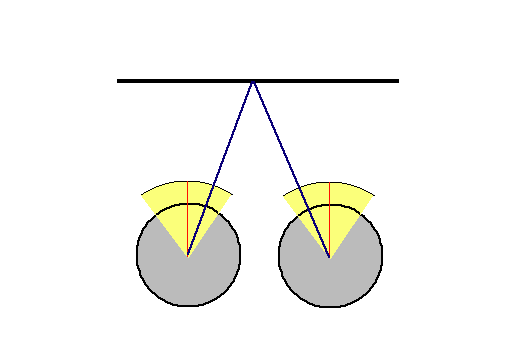
\includegraphics[width=0.7\textwidth]{./images/chapter5/different_angle_cover_example.png}
    \caption{Παράδειγμα Κάλυψης Σημείου υπό Διαφορετικών Γωνιών}
    \label{fig:different_angle_cover_example}
\end{figure}

Συμπερασματικά, η κάθε κάλυψη μπορεί να ποσοτικοποιηθεί στις παρακάτω πέντε μετρικές, οι οποίες και χρησιμοποιήθηκαν σε όλα τα πειράματα κάλυψης χώρου.
\begin{itemize}
    \setlength\itemsep{-0.2em}
    \item Ποσοστό συνολικής κάλυψης των εμποδίων του χώρου
    \item Μέση τιμή πλήθους σαρώσεων κάθε σημείου
    \item Διακύμανση πλήθους σαρώσεων κάθε σημείου
    \item Μέση τιμή μετρικής γωνίας σάρωσης κάθε σημείου που έχει σαρωθεί
    \item Διακύμανση μετρικής γωνίας σάρωσης κάθε σημείου που έχει σαρωθεί
\end{itemize}


Η υλοποίηση του συστήματος αυτού περιλαμβάνει δύο συναρτήσεις. Η πρώτη \ref{alg:circular_ray_cast_coverage} είναι αυτή που βρίσκει τα σημεία του OGM που καλύπτονται κάθε φορά από έναν αισθητήρα του ρομποτικού οχήματος. Για δεδομένα χαρακτηριστικά αισθητήρα και πόζα του οχήματος υπολογίζονται τα σημεία με τη χρήση του brushfire αλγορίθμου και της ray casting τεχνικής. Συγκεκριμένα, δημιουργείται μια ακτίνα από την κεραία προς τα έξω, πάνω στην οποία εκτελείται ο αλγόριθμος brushfire μέχρι να συναντήσει εμπόδιο ή να ξεπεράσει την ακτίνα κάλυψης του αισθητήρα. Όλα τα ελεύθερα σημεία στα οποία διαδίδεται ο brushfire είναι αυτά που καλύπτει ο αισθητήρας. Η διαδικασία αυτή εκτελείται επαναληπτικά για όλες τις ακτίνες μέσα στο FOV του αισθητήρα με πολύ μικρό βήμα, ίσο με $0.5$ μοίρες. Επίσης, υπάρχει η επιλογή μέσω της μεταβλητής εισόδου $return\_obstacles$ ο αλγόριθμος να επιστρέψει είτε τα σημεία του ελεύθερου χώρου είτε το σύνολο των εμποδίων που σαρώνονται. 

Η μέθοδος αυτή φέρει σημαντικά πλεονεκτήματα. Συγκεκριμένα, με τη χρήση του brushfire, η εξάπλωση περιορίζεται αποκλειστικά στον γύρω ελεύθερο χώρο και δεν σαρώνονται τα σημεία εμποδίων. Πράγματι, η εξάπλωση σταματάει για κάθε ακτίνα μόλις εντοπιστεί εμπόδιο και παραμένει στο ίδιο δωμάτιο. Συνεπώς, δεν σαρώνονται σημεία πίσω από τοίχους, κάτι που ρεαλιστικά οι αισθητήρες αδυνατούν να κάνουν. Επιπλέον, η χρήση της ray casting τεχνικής προσομοιώνει την πραγματική λειτουργία του αισθητήρα, καθώς αυτός σαρώνει σε συγκεκριμένο πεδίο ενός κύκλου το οποίο μπορεί να προσεγγιστεί ικανοποιητικά χρησιμοποιώντας ένα μεγάλο πλήθος ακτίνων.

Ο \autoref{alg:update_cover} συντονίζει τη διαδικασία κάλυψης. Διαβάζει, αρχικά, την τρέχουσα θέση του οχήματος και ελέγχει εαν αυτό έχει κινηθεί, συγκρίνοντας την με την προηγούμενη μέτρηση. Αυτός ο έλεγχος γίνεται για εξοικονόμηση υπολογιστικής ισχύος, καθώς όταν το όχημα παραμένει ακίνητο οι αισθητήρες εντοπίζουν τα ίδια σήματα. Εαν το ρομπότ έχει κινηθεί ως προς οποιαδήποτε από τις τρεις μεταβλητές υπολογίζονται τα σημεία που καλύπτει το σύνολο των αισθητήρων του. Μετά, για κάθε σημείο ανανεώνεται η τιμή κάλυψης του στον πίνακα $coverage$, ο οποίος έχει διαστάσεις ίσες με το OGM του χώρου και αποθηκεύει την κάλυψη ή όχι του κάθε διακριτού σημείου με τιμές $100$ και $0$, αντίστοιχα. Επίσης, ανανεώνεται η τιμή πλήθους σαρώσεων στον $coverage\_number$, αλλά και του πλήθους σαρώσεων κάθε τμήματος γωνιών στον $coverage\_angles$, έναν τρισδιάστατο πίνακα με τρίτη διάσταση ίση με 2. 

Ένα παράδειγμα του πίνακα $coverage$ παρουσιάζεται στο \ref{fig:coverage_ogm_example}, όπου φαίνεται το OGM του περιβάλλοντος και με σκούρο γκρι χρώμα είναι σημειωμένα όλα τα σημεία τα οποία καλύφθηκαν από τους αισθητήρες κατά την πλοήγηση του στον χώρο. 


\begin{figure}[!htb]
    \centering
    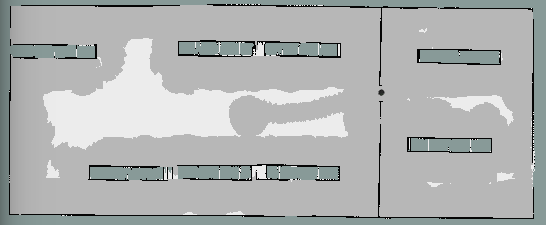
\includegraphics[width=0.8\textwidth]{./images/chapter5/warehouse_4_wall_follow_a_priori_coverage_085_weights_1_2_real.png}
    \caption{Παράδειγμα Πεδίου Κάλυψης}
    \label{fig:coverage_ogm_example}
\end{figure}

\begin{algorithm}[H]
\caption{Circular Ray Cast Coverage}
\label{alg:circular_ray_cast_coverage}
\begin{algorithmic}[1]
    \Function{circularRayCastCoverage}{start, ogm, cover\_range, fov, theta, direction, return\_obstacles = False}
    \State $brushfire = numpy.zeros(ogm.shape, np.dtype('int32'))$
    \State $brushfire[ogm > 49] = 1$
    \State $brushfire[ogm == -1] = -1$
    \State $brushfire[start] = 2$
    \State $th = -fov/2$
    \While{$th <= fov/2$}
        \State $angle = (th + direction + theta) *  $ π $/ 180.0;$
        \State $step = 2$, $iters = 1$
        \While{$iters <= cover\_length$}
            \State $xx = (int) round(start[0] + cos(angle) * iters)$
            \State $yy = (int) round(start[1] + sin(angle) * iters)$
            \If{$brushfire[xx][yy] == 0$}
                \State $brushfire[xx][yy] = step$
                \State $step++$
            \ElsIf{$brushfire[xx][yy] == 1$}
                \State $brushfire[xx][yy] = -2$
                \State break
            \ElsIf{$brushfire[xx][yy] < 0$}
                \State break
            \EndIf
            \State $iters++$
        \EndWhile
        \State $th += 0.5$
    \EndWhile
    \If{return\_obstacles}
        \State $indexes = zip(*numpy.where(brushfire == -2))$
    \Else
        \State $indexes = zip(*numpy.where(brushfire > 1))$
    \EndIf
    \State \Return $indexes$
\end{algorithmic}
\end{algorithm}


\begin{algorithm}[H]
\caption{Update Cover}
\label{alg:update_cover}
\begin{algorithmic}[1]
    \Function{updateCover}{previous\_robot\_pose, ogm, coverage, coverage\_number, coverage\_angles, resolution,  sensor\_range, sensor\_fov, sensor\_direction}
    \State Read robot's pose $xx$, $yy$, $th$
    \State Check if robot has been moved from previous pose 
    \If{robot moved}
        \For{each sensor $s$}
            \State $cover\_length = int(sensor\_range[s] / resolution)$
            \State $indexes = circularRayCastCoverage((xx,yy), ogm, cover\_length,$\par
            \hskip\algorithmicindent $sensor\_fov[s], th, sensor\_direction[s])$
            \For{$x$, $y$ in $indexes$}
                \State $coverage[x, y] = 100$
                \State $coverage\_number[x, y] += 1$
                \State $angle = th + sensor\_direction[s] + math.degrees(math.atan2(yy-y,xx-x))$
                \If{$angle < 0$}
                    \State $coverage\_angles[x, y][0] += 1$
                \Else
                    \State $coverage\_angles[x, y][1] += 1$
                \EndIf
            \EndFor
        \EndFor
    \EndIf
    \State  Update $previous\_robot\_pose$ with current pose
    \State \Return $coverage$, $coverage\_number$, $coverage\_angles$, $previous\_robot\_pose$
\end{algorithmic}
\end{algorithm}


\section{Βελτιστοποίηση Μονοπατιού Κάλυψης Δωματίου}
\label{section:room_path_implementation}

Το τελευταίο και μεγαλύτερο τμήμα της εργασίας αυτής είναι η πλήρης κάλυψη κάθε δωματίου. Για να επιτευχθεί αυτό χρειάζεται να υπολογιστούν σημεία στα οποία θα κατευθυνθεί το ρομποτικό όχημα σαρώνοντας, έτσι, έμμεσα τον χώρο. Όλοι οι υπολογισμοί πραγματοποιούνται συναρτήσει των αισθητήρων. Υλοποιήθηκαν δύο διαφορετικές στρατηγικές, η στρατηγική ακολουθίας τοίχων και η στρατηγική ζιγκ ζαγκ. Η διαδικασία αυτή αποτελείται από τα παρακάτω βήματα:

\begin{itemize}
    \setlength\itemsep{-0.2em}
    \item Δειγματοληπτικός υπολογισμός σημείων κάλυψης
    \item Υπολογισμός βέλτιστης αλληλουχίας επίσκεψης των σημείων
    \item Υπολογισμός βέλτιστου προσανατολισμού σε κάθε σημείο
    \item Προσομοίωση κάλυψης του χώρου και διαγραφή περιττών σημείων
    \item Δημιουργία αλληλουχίας κόμβων ζιγκ-ζαγκ
\end{itemize}

\subsection{Δειγματοληπτικός υπολογισμός σημείων κάλυψης}
\label{subsection:nodes_sampling}

Αρχικά, πρέπει να εξαχθεί ένα σύνολο σημείων στα οποία πηγαίνοντας το όχημα θα έχει την δυνατότητα να καταγράψει προϊόντα, δηλαδή σημεία που βρίσκονται κοντά σε εμπόδια. Το πόσο κοντά, φυσικά, εξαρτάται από την ακτίνα των κεραιών RFID που φέρει το ρομπότ.

Η μέθοδος που υλοποιήθηκε εφαρμόζει ομοιόμορφη δειγματοληψία επαναληπτικά μεταβάλλοντας το βήμα της και αποθηκεύει όλα τα σημεία τα οποία βρίσκονται σε κοντινή απόσταση από τα γύρω εμπόδια. Το κέρδος με την χρήση πολλών διαφορετικών βημάτων είναι ότι αποθηκεύονται σημεία σε όλο τον ελεύθερο χώρο που μπορεί να επισκευτεί το ρομπότ ανεξαρτήτως της τοπολογίας του. 

Πρώτα υπολογίζονται η ελάχιστη και η μέγιστη τιμή των ακτίνων των διάφορων κεραιών που φέρει το ρομπότ. Μετά, επαναληπτικά σαρώνεται ολόκληρος ο χάρτης με κάποιο βήμα και κρατούνται όλα εκείνα τα σημεία που βρίσκονται στον ελεύθερο χώρο και απέχουν απόσταση από τα γύρω εμπόδια στο διάστημα $(step, 2*step]$. Θέτοντας αυτόν τον περιορισμό, σε κάθε επανάληψη σχηματίζεται μόλις μία σειρά σημείων εσωτερικά των εμποδίων και όχι περισσότερες, κάτι που οδηγεί σε μεγάλο πλεόνασμα σημείων μέσα στην ίδια επανάληψη. Το \autoref{fig:sampling_double_points_example} αποτελεί μια περίπτωση περισσότερων της μίας σειράς σημείων. Φυσικά, για να γίνει δεκτό ένα σημείο πρέπει οι κεραίες να είναι επαρκώς κοντά σε κάποιο εμπόδιο.


\begin{figure}[!htb]
    \centering
    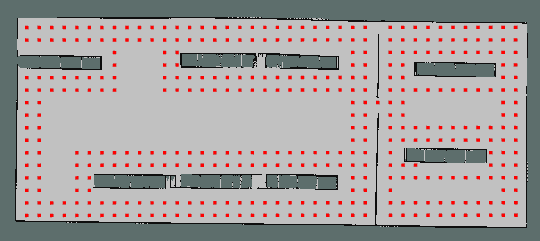
\includegraphics[width=0.8\textwidth]{./images/chapter5/sampling_double_points_example.png}
    \caption{Παράδειγμα Αποτυχίας Εύρεσης Σημείων}
    \label{fig:sampling_double_points_example}
\end{figure}


Το βήμα της δειγματοληψίας αρχίζει από τιμή ίση με μιάμιση φορά την ακτίνα του οχήματος, όσο δηλαδή και η ελάχιστη απόσταση που μπορεί να φτάσει το όχημα από τα εμπόδια για λόγους ασφαλείας και διπλασιάζεται σε κάθε επανάληψη μέχρι να γίνει μεγαλύτερο από την μέγιστη ακτίνα των κεραιών. Ένα τέτοιο παράδειγμα για τα σημεία με διαφορετικό βήμα δειγματοληψίας παρουσιάζεται στο \ref{fig:sampling_steps_examples}. Έτσι, όμως, θα υπάρχουν πολλά σημεία απ' όπου το ρομπότ θα σαρώσει τα ίδια εμπόδια, είναι δηλαδή περιττά. Επομένως, πρέπει να γίνει ένας τελικός έλεγχος εαν κάθε σημείο προσφέρει όντως στην κάλυψη, δίνοντας προτεραιότητα στα σημεία που προέκυψαν από την δειγματοληψία με τα μεγαλύτερα βήματα. Για κάθε σημείο υπολογίζονται τα εμπόδια που μπορούν να σαρωθούν από εκεί και εαν περισσότερα από το 90\% τους έχουν ήδη καλυφθεί από τα προηγούμενα, τότε αυτό απορρίπτεται. Σημειώνεται ότι τα σημεία που προέκυψαν από το μεγαλύτερο βήμα δειγματοληψίας κρατούνται όλα. Με τη μέθοδο αυτή εξασφαλίζεται ότι θα αποθηκευτούν τελικά τα λιγότερα δυνατά σημεία που καλύπτουν ολόκληρο τον χώρο. Ο αλγόριθμος περιγράφεται αναλυτικά στο \ref{alg:uniform_sampling}.


\begin{algorithm}[!htb]
\caption{Uniform Sampling}
\label{alg:uniform_sampling}
\begin{algorithmic}[1]
    \Function{uniformSampling}{brush, sensor\_range, resolution, robot\_radius}
    \State $nodes = [], step\_list = []$
    \State $min\_range = int(min(sensor\_range)/resolution)$
    \State $max\_range = int(max(sensor\_range)/resolution)$
    \State $step = int(1.5 * robot\_radius / resolution)$
    \While{$step <= max\_range$} 
        \State $temp\_nodes = []$
        \State $step\_list.append(step)$
        \State $indexes = np.where((brush > step)\ \&\ (brush <= 2*step)\ \&\ (brush <= max\_range))$
        \State $indexes = zip(*indexes)$
        \For{each $(x,y)$ in $indexes$}
            \If{not $x\ \%\ step$ and not $y\ \%\ step$}
                \State $temp\_nodes.append((x,y))$
            \EndIf
        \EndFor
        \State $step *= 2$
        \State $nodes.append(temp\_nodes)$
    \EndWhile
    \State $obstacles = numpy.zeros(brush.shape), final\_nodes = [], i = len(nodes) - 1$
    \While{$i >= 0$}
        \State $temp\_nodes = nodes[i]$
        \State \Comment{Check if new nodes override previous ones and delete them}
        \For{$point$ in $temp\_nodes$}
            \State $indexes = circularRayCastCoverage(point, ogm, max\_range,$ \par
            \hskip \algorithmicindent $360, 0, 0, True)$
            \If{not $len(indexes)$}
                \State continue
            \ElsIf{$i == len(nodes) - 1$}
                \State $obstacles[zip(*indexes)] = 1$
                \State $final\_nodes.append(point)$
            \Else
                \State $temp = obstacles[zip(*indexes)]$
                \State $p = len(np.where(temp > 0)[0]) / len(indexes)$
                \If{$p<0.9$}
                    \State $final\_nodes.append((x,y))$
                    \State $obstacles[zip(*indexes)] = 1$
                \EndIf
            \EndIf
        \EndFor
        \State $i -= 1$
    \EndWhile
    \State \Return $final\_nodes, step\_list$
\end{algorithmic}
\end{algorithm}


\begin{figure}
     \centering
     \begin{subfigure}[b]{\textwidth}
         \centering
         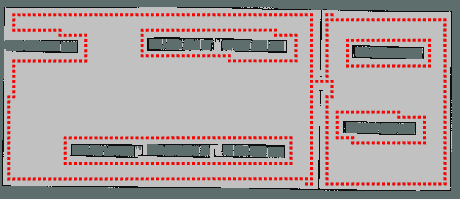
\includegraphics[width=0.8\textwidth]{./images/chapter5/warehouse_4_sampling_steps_1.png}
         \label{fig:warehouse_4_sampling_steps_1}
     \end{subfigure}
     \hfill
     \begin{subfigure}[b]{\textwidth}
         \centering
         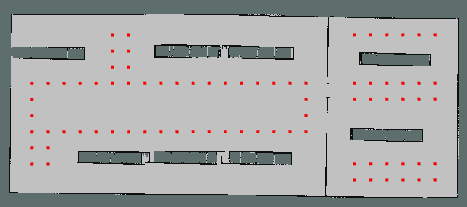
\includegraphics[width=0.8\textwidth]{./images/chapter5/warehouse_4_sampling_steps_2.png}
         \label{fig:warehouse_4_sampling_steps_2}
     \end{subfigure}
     \hfill
     \begin{subfigure}[b]{\textwidth}
         \centering
         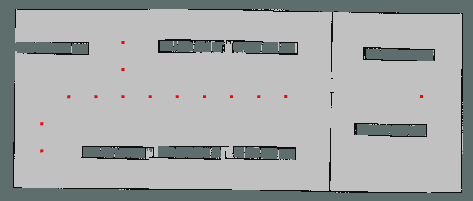
\includegraphics[width=0.8\textwidth]{./images/chapter5/warehouse_4_sampling_steps_3.png}
         \label{fig:warehouse_4_sampling_steps_3}
     \end{subfigure}
    \caption{Δειγματοληψία με διάφορα βήματα}
    \label{fig:sampling_steps_examples}
\end{figure}


Αντίθετα, εαν γίνει χρήση σταθερού βήματος δειγματοληψίας είναι πολύ πιθανό να προκύψουν περιοχές χωρίς σημεία πράγμα που σημαίνει αποτυχία πλήρους κάλυψης του χώρου, όπως φαίνεται και στο σχήμα \ref{fig:wrong_sampling_example}.


\begin{figure}[!htb]
    \centering
    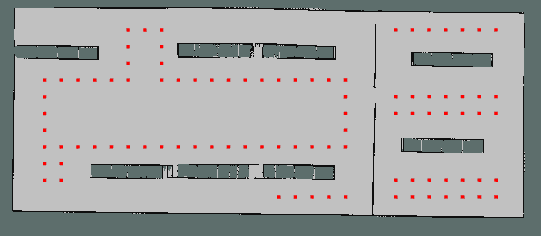
\includegraphics[width=0.8\textwidth]{./images/chapter5/range_2_get_only_in_second_half.png}
    \caption{Παράδειγμα Αποτυχίας Εύρεσης Σημείων}
    \label{fig:wrong_sampling_example}
\end{figure}




\subsection{Υπολογισμός βέλτιστης αλληλουχίας επίσκεψης των σημείων}
\label{subsection:node_sequence_optimization}

Στην συνέχεια, τα σημεία αυτά χωρίζονται στα διάφορα δωμάτια και υπολογίζεται η βέλτιστη αλληλουχία των σημείων ανά δωμάτιο. Η διαδικασία αυτή έχει τα παρακάτω βήματα.

\begin{itemize}
    \setlength\itemsep{-0.2em}
    \item Διαχωρισμός σημείων σε δωμάτια
    \item Hill Climbing σε συνδιασμό με τον αλγόριθμο κοντινότερου γείτονα
    \item Προσθήκη των πορτών εισόδου και εξόδου του δωματίου στην αλληλουχία
    \item RRHC με τις πόρτες σταθερές στις άκρες της αλληλουχίας
\end{itemize}

Ο διαχωρισμός των κόμβων σε δωμάτια πραγματοποιείται χωρίζοντας το OGM σε ασύνδετους χώρους, δηλαδή προσθέτοντας τοίχους εκεί που υπάρχουν οι πόρτες και χρησιμοποιώντας μια παραλλαγή του αλγορίθμου brushfire, την \emph{pointBrushfire}. 

Οι πόρτες του χώρου είναι ήδη γνωστές ενώ τα κοντινότερα εμπόδια τους, δηλαδή οι δύο τοίχοι υπολογίζονται από τον αλγόριθμο \emph{closestObstacleBrushfire} \ref{alg:closestObstacleBrushfire}. Στη συνέχεια, υπολογίζεται η νοητή ευθεία του τοίχου, δηλαδή η ευθεία της κάθε πόρτας στο OGM και προστίθεται τοίχος, δηλαδή τα σημεία αυτά τίθονται ίσα με $100$ στο νέο OGM. Η συνάρτηση αυτή παρουσιάζεται στο \ref{alg:door_closure}.

\begin{algorithm}[!htb]
\caption{Door Closure}
\label{alg:door_closure}
\begin{algorithmic}[1]
    \Function{doorClosure}{doors, ogm}
    \State $filled\_ogm = numpy.copy(ogm)$
    \For{$door$ in $doors$}
        \State $ob = closestObstacleBrushfire(door, ogm)$
        \State Find obstacle points' line
        \State Set points of line equal to $100$ in $filled\_ogm$
    \EndFor
    \State \Return $filled\_ogm$
\end{algorithmic}
\end{algorithm}


Έπειτα, με την χρήση brushfire με αρχή τους κόμβους κάθε δωματίου από την προηγούμενη διαδικασία εξαγωγής χρήσιμων σημείων από το GVD \ref{subsection:find_room_nodes} και το διαχωρισμένο σε δωμάτια OGM χωρίζονται οι κόμβοι προσπέλασης σε δωμάτια.

Στη συνέχεια, για κάθε δωμάτιο υπολογίζεται μια βέλτιστη αλληλουχία. Τα σημεία ταξινομούνται σύμφωνα με τις συντεταγμένες τους $(x,y)$ και στη συνέχεια χρησιμοποιείται μια παραλλαγή του HC που αξιοποιεί το γεγονός ότι η δειγματοληψία των σημείων έχει πραγματοποιηθεί με συγκεκριμένα βήματα. Αυτό σημαίνει ότι τα σημεία που είναι πολύ κοντά μεταξύ τους, θα έχουν απόσταση ίση με ένα από τα διάφορα βήματα, τα οποία έχουν αποθηκευτεί στο $step\_list$ στον αλγόριθμο \ref{alg:uniform_sampling}. Έτσι, υπολογίζεται μια αλληλουχία με βάση εαν τα σειριακά σημεία έχουν μεταξύ τους απόσταση ίση με τα βήματα της δειγματοληψίας. Εαν δεν υπάρχει τέτοιο σημείο, τότε προστίθεται στην σειρά το κοντινότερο δυνατό, χρησιμοποιείται, δηλαδή, και η προσέγγιση του κοντινότερο γείτονα. Ο αλγόριθμος που περιγράφει αυτή την διαδικασία παρουσιάζεται στο \ref{alg:step_hillclimb}.



\begin{algorithm}[!htb]
\caption{Step Hill Climb}
\label{alg:step_hillclimb}
\begin{algorithmic}[1]
    \Function{stepHillClimb}{distances, epochs, steps}
    \State $length = distances.shape[0]$
    \State $best = range(length)$
    \State Set $best\_score$ equal to the length of route $best$
    \State $iter = 0$
    \For{$i$ in $range(length-2)$}
        \If{$iter >= epochs$}
            \State break
        \EndIf
        \State $minimum = distances[best[i]][best[i+1]]$
        \If{$minimum <= min(steps)$}
            \State continue
        \Else
            \State Find point $index$ closest to point $i$
            \State $best[i+1], best[index] = best[index], best[i+1]$
            \State Set $best\_score$ equal to the length of route $best$
        \EndIf
    \EndFor
    \State \Return $best, best\_score, iter$
\end{algorithmic}
\end{algorithm}

Στη συνέχεια, προστίθενται και οι πόρτες εισόδου και εξόδου στην αρχή και στο τέλος αντίστοιχα της υπολογισμένης αλληλουχίας. Μάλιστα, για την περαιτέρω βελτίωση της, πραγματοποιείται μια εσωτερική κυκλική περιστροφή των σημείων, έτσι ώστε το δεύτερο σημείο να είναι το κοντινότερο από την πόρτα εισόδου που είναι το πρώτο σημείο. Αυτή είναι μια λογική μεταβολλή η οποία βελτιώνει την συνολική απόσταση του μονοπατιού χωρίς την χρήση σύνθετων αλγορίθμων.

Τέλος, εφαρμόζεται ο RRHC αλγόριθμος με σταθερά άκρα τις πόρτες εισόδου και εξόδου στο δωμάτιο. Μετά από πειραματισμούς στο πλήθος των επαναλήψεων του RRHC με τιμές 1000, 2000 και 5000 φορές επί το πλήθος των σημείων του δωματίου, προέκυψε ότι ιδανικότερος αριθμός είναι οι 2000 επί πλήθος των σημείων του δωματίου. Είναι ένας αριθμός που φέρει πολύ καλά αποτελέσματα χωρίς να απαιτεί σημαντικό χρόνο υπολογισμών. Ο RRHC αναλύεται στο \ref{alg:rrhc}.


Ένα παράδειγμα της προόδου του μήκους της αλληλουχίας των διάφορων δωματίων ενός χάρτη σε κάθε ένα από τα τέσσερα στάδια επεξεργασίας παρουσιάζεται στον επόμενο πίνακα \ref{tab:room_path_length_stages_optimization} και στα σχήματα \ref{fig:wall_follow_optimization_example}. Η μελέτη πραγματοποιήθηκε στο το OGM του σχήματος \ref{fig:wf_opt_ogm}, πάνω στο οποίο εμφανίζεται και με κόκκινους αριθμούς η σειρά των δωματίων. Η σειρά επίσκεψης των σημείων κάθε δωματίου οπτικοποιείται με την εναλλαγή χρωμάτων ανά δωμάτιο. Το όχημα θα εκκινεί από τα σκούρα σημεία και θα κατευθύνεται στα πιο ανοικτόχρωμα, καταλήγοντας στα άσπρα.


\begin{table}[H]
    \begin{center}
        \caption{Βελτίωση μήκους διαδρομής ανά στάδιο επεξεργασίας}
        \label{tab:room_path_length_stages_optimization}
        \begin{tabular}{|>{\columncolor[gray]{0.8}} c | c | c | c | c | c | c |}
        \hline
        \rowcolor{gray}
        Stages & room 1 & room 2 & room 3 & room 4 & room 5 & room 6 \\
        \hline
        sort & 14719 & 4711 & 5398 & 4699 & 4443 & 2633 \\ 
        \hline
        stepHC & 3951 & 1494 & 1049 & 945 & 1275 & 1024 \\
        \hline
        adding doors & 4554 & 1524 & 1060 & 1212 & 1283 & 1056 \\ 
        \hline
        RRHC & 3761 & 1344 & 935 & 1032 & 1131 & 944 \\ 
        \hline
        \end{tabular}
    \end{center}
\end{table}

\begin{figure}
    \centering
    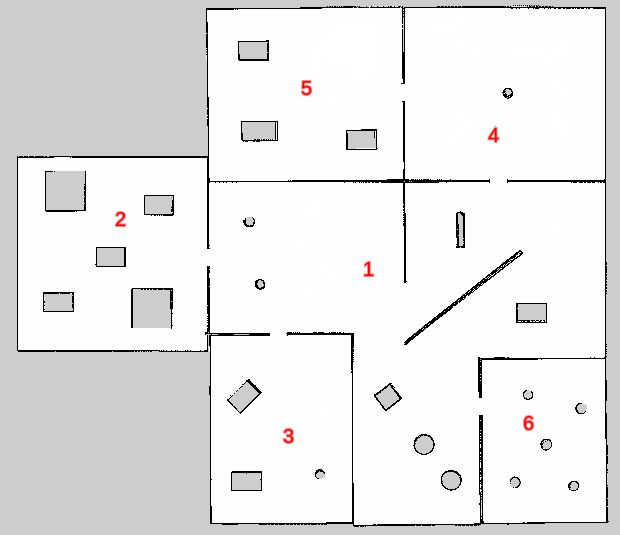
\includegraphics[width=0.5\textwidth]{./images/chapter5/wf_opt_ogm.png}
    \caption{Περιβάλλον ελέγχου διαδικασίας υπολογισμού μονοπατιού}
    \label{fig:wf_opt_ogm}
\end{figure}



\begin{figure}[!htb]
     \centering
     \begin{subfigure}[b]{0.5\textwidth}
         \centering
         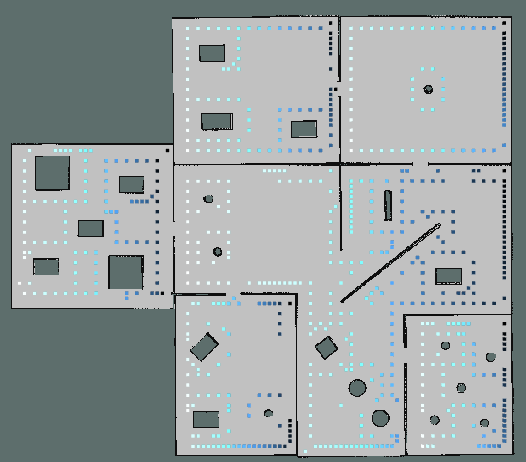
\includegraphics[width=0.9\textwidth]{./images/chapter5/wf_optimization_1_sorted.png}
         \label{fig:wf_optimization_1_sorted}
         \caption{sort}
     \end{subfigure}%
    %  \hfill
     \begin{subfigure}[b]{0.5\textwidth}
         \centering
         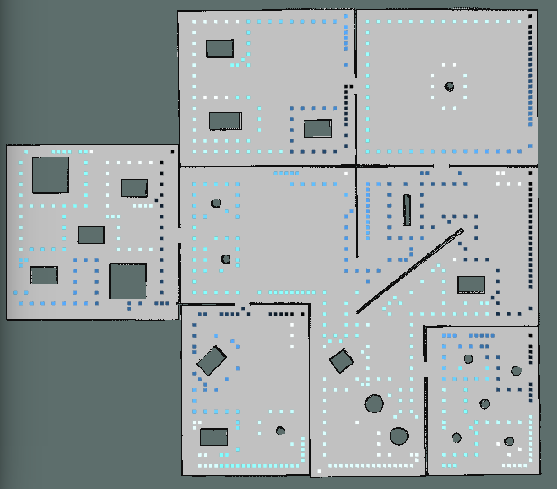
\includegraphics[width=0.9\textwidth]{./images/chapter5/wf_optimization_2_stepHC.png}
         \label{fig:wf_optimization_2_stepHC}
         \caption{stepHC}
     \end{subfigure}
     \hfill
     \begin{subfigure}[b]{0.5\textwidth}
         \centering
         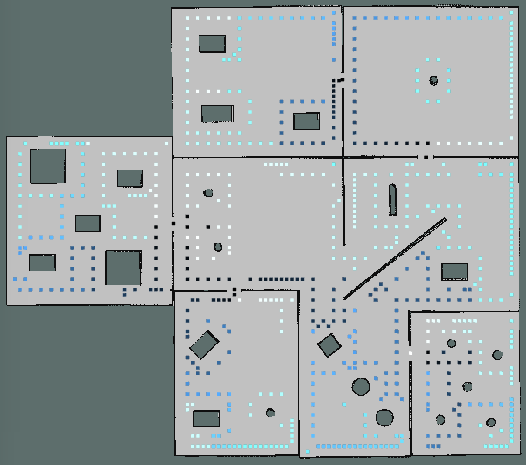
\includegraphics[width=0.9\textwidth]{./images/chapter5/wf_optimization_3_added_doors.png}
         \label{fig:wf_optimization_3_added_doors}
         \caption{adding doors}
     \end{subfigure}%
    %  \hfill
     \begin{subfigure}[b]{0.5\textwidth}
         \centering
         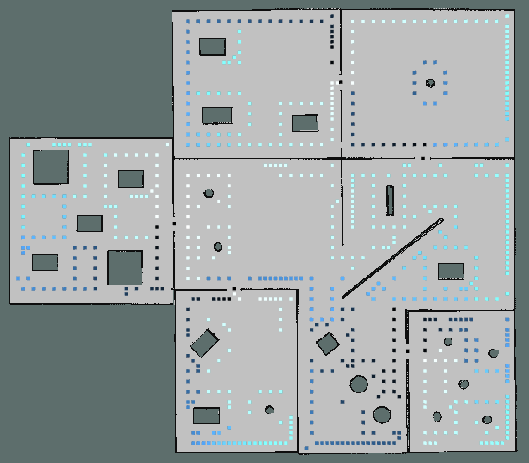
\includegraphics[width=0.9\textwidth]{./images/chapter5/wf_optimization_4_rrhc.png}
         \label{fig:wf_optimization_4_rrhc}
         \caption{RRHC}
     \end{subfigure}
    \caption{Στάδια βελτίωσης μονοπατιού}
    \label{fig:wall_follow_optimization_example}
\end{figure}



\subsection{Υπολογισμός βέλτιστου προσανατολισμού σε κάθε σημείο}
\label{subsection:find_pose}

Αφότου βρεθεί το σύνολο των σημείων για την πλήρη κάλυψη του χώρου, χρειάζεται να υπολογιστεί και η βέλτιστη γωνία του ρομπότ σε κάθε θέση. Άλλωστε, η ακριβής θέση του οχήματος στον διδιάστατο χώρο αποτελείται από τρεις μεταβλητές, δύο για την θέση και μία για τον προσανατολισμό. Τα κριτήρια επιλογής του προσανατολισμού είναι δύο. Το πρώτο είναι οι αισθητήρες να καλύπτουν όσο το δυνατόν περισσότερη επιφάνεια εμποδίων και το δεύτερο η γωνιακή μετατόπιση ανάμεσα στον τρέχοντα προσανατολισμό και το επόμενο σημείο να είναι η ελάχιστη δυνατή. Αυτά μας εξασφαλίζουν όσο το δυνατόν μεγαλύτερη κάλυψη του χώρου και ελαχιστοποίηση της χρονικής διάρκειας της διαδικασίας αντίστοιχα. Για τον λόγο αυτό δημιουργήθηκε μια συνδιαστική συνάρτηση των δύο αυτών παραμέτρων με την μέθοδο motor schema, όπου λαμβάνονται υπόψη και οι δύο παράμετροι με κάποιο βάρος. Η μέθοδος υπολογισμού των βαρών αυτών παρουσιάζεται στο τέλος της υποενότητας.

Πρώτα αναλύεται η διαδικασία επιλογής κάθε γωνίας στροφής. Για κάθε σημείο στόχο εξετάζονται όλες οι γωνίες μία προς μία με βήμα 10 μοιρών και κρατείται αυτή που δίνει την βέλτιστη τιμή της συνάρτησης του motor schema, η οποία είναι η παρακάτω.

\[eval = obstacle\_weight * \frac{len(covered\_obstacles)}{len(obstacles)} + rotation\_weight * \frac{180 - next\_rotation}{180}\]

Ο πρώτος όρος περιέχει το πλήθος των εμποδίων που καλύπτονται από την εν λόγω γωνία και ο δεύτερος περιέχει τη γωνιακή στροφή προς το επόμενο σημείο στόχο. Και οι δύο είναι κανονικοποιημένοι, έτσι ώστε οι τιμές να περιορίζονται στο εύρος $[0,1]$ και το $1$ να αντιστοιχεί στο βέλτιστο επιμέρους αποτέλεσμα. 

Σε κάθε σημείο, όμως, δεν αποθηκεύεται μόνο μια γωνία αλλά μπορούν και περισσότερες μέχρι να έχει συνολικά καλυφθεί το περισσότερο τμήμα των γύρω εμποδίων, δηλαδή ένα ποσοστό μεγαλύτερο του 50\%. Μετά από ορισμένες δοκιμές βρέθηκε ότι το όριο του 60\% προσφέρει καλή συνολική κάλυψη του χώρου. Mεγαλύτερα όρια, όπως τα 75\% και 80\%, οδηγούν σε αποθήκευση πολλών περιττών θέσεων - στόχων χωρίς βελτίωση στην συνολική τελική κάλυψη του χώρου, ενώ το μικρότερο όριο 50\% οδηγεί σε μείωση της κάλυψης. Συνεπώς, για κάθε σημείο αποθηκεύονται οι καλύτερες γωνίες εως ότου έχει καλυφθεί τουλάχιστον το 60\% των κοντινών εμποδίων. Το ποσοστό είναι φαινομενικά μικρό, ωστόσο εξαιτίας της κοντινής απόστασης μεταξύ των σημείων στόχων οδηγεί σε θεμιτά αποτελέσματα. 

Αυτό το κατώφλι χρησιμοποιήθηκε για τις περιπτώσεις που υπάρχουν περισσότερα του ενός εμπόδια στην γύρω περιοχή και το όχημα φέρει μικρό αριθμό αισθητήρων, για παράδειγμα έναν. Τότε εαν αποθηκευτεί ένας μόνο στόχος, είναι πολύ πιθανό να μην σαρωθεί σημαντικό τμήμα των εμποδίων. Με την πολλαπλή αποθήκευση γωνιών σε κάθε σημείο εξασφαλίζεται η καλύτερη δυνατή κάλυψη της κάθε περιοχής. Ο αλγόριθμος αυτός παρουσιάζεται αναλυτικά στο \ref{alg:find_best_yaw}.  

\begin{algorithm}[!h]
\caption{Find Best Yaw}
\label{alg:find_best_yaw}
\begin{algorithmic}[1]
    \Function{findBestYaw}{node, next\_node, obstacle\_weight, rotation\_weight, sensor\_range, resolution}
        \State $yaw = []$
        \State $yaw\_between\_nodes = math.degrees(math.atan2(next\_node[1]-node[1], next\_node[0]-node[0]))$
        \State $steps = int(max(sensor\_range) / resolution)$
        \State Fill $obstacles$ with indexes of nearby obstacles at range $steps$
        \State $found = 0$
        \While{$found < 0.6 * len(obstacles)$ and $len(obstacles)$}
            \State $best\_evaluation = 0$, $best\_yaw = 0$, $best\_found = 0$, $best\_covered\_obstacles = []$
            \For{each angle $angle$ in $[-180, 180]$}
                \State Check covered nearby obstacles $covered\_obstacles$
                \State $next\_rotation = abs(angle - yaw\_between\_nodes)$
                \State Evaluate candidate angle
                \If{$angle$ is better than current best}
                    \State $best\_evaluation = angle$'s evaluation
                    \State $best\_yaw = angle$
                    \State $best\_found = len(covered\_obstacles)$ 
                    \State $best\_covered\_obstacles = covered\_obstacles$
                \EndIf
            \EndFor
            \State $found += best\_found$
            \State Discard $best\_covered\_obstacles$ from $obstacles$
        \EndWhile
        \State \Return $best\_yaw$
\end{algorithmic}
\end{algorithm}



Τέλος, η διαδικασία αυτή υλοποιήθηκε σε έναν συγκεκριμένο χάρτη με πέντε διαφορετικούς συνδιασμούς βαρών, ώστε να μελετηθεί η επιρροή τους και να επέλθει η τελική μέθοδος επιλογής τους στην προηγούμενη συνάρτηση. Μελετήθηκαν η εκτίμηση της κάλυψης του χώρου, η πραγματική κάλυψη του και ο χρόνος της και τα αποτελέσματα παρουσιάζονται στους επόμενους δύο πίνακες \ref{tab:motor_schema_weights_side_antennas}, \ref{tab:motor_schema_weights_front_back_antennas} για διαφορετικούς αισθητήρες. Στην πρώτη περίπτωση οι κεραίες είναι τοποθετημένες στα πλάγια του οχήματος, ενώ στην δεύτερη στο μπροστά και το πίσω μέρος του. 

\begin{table}[H]
    \centering
    \begin{tabular}{|>{\columncolor[gray]{0.8}} c | >{\columncolor[gray]{0.8}} c  | c | c | c |}
        \hline
             Obstacle W.  & Rotation W. & Εκτίμηση  & Πραγματική Κάλυψη & Χρόνος  \\
             \hline
             $4$ & $1$ & $85.49$ \% & $87.43$ \% & 71.6 min \\
             $2$ & $1$ & $85.80$ \% & $85.95$ \% & 71.2 min \\
             $1$ & $1$ & $85.04$ \% & $86.78$ \% & 66 min \\
             $1$ & $2$ & $83.16$ \% & $86.20$ \% & 59.5 min \\
             $1$ & $4$ & $83.16$ \% & $86.74$ \% & 76.6 min \\
        \hline
    \end{tabular}
    \caption{Εκτίμηση Βαρών Motor Schema με Κεραίες στα Πλάγια}
    \label{tab:motor_schema_weights_side_antennas}
\end{table}

\begin{table}[H]
    \centering
    \begin{tabular}{|>{\columncolor[gray]{0.8}} c | >{\columncolor[gray]{0.8}} c  | c | c | c |}
        \hline
             Obstacle W.  & Rotation W. & Εκτίμηση  & Πραγματική Κάλυψη & Χρόνος  \\
             $4$ & $1$ & $85.95$ \% & $83.03$ \% & 76 min \\
             $2$ & $1$ & $85.34$ \% & $83.61$ \% & 73.7 min \\
             $1$ & $1$ & $84.85$ \% & $80.58$ \% & 66.4 min \\
             $1$ & $2$ & $83.29$ \% & $84.38$ \% & 98.18 min \\
             $1$ & $4$ & $82.81$ \% & $85.41$ \% & 122.1 min \\
        \hline
    \end{tabular}
    \caption{Εκτίμηση Βαρών Motor Schema με Κεραίες Μπροστά και Πίσω}
    \label{tab:motor_schema_weights_front_back_antennas}
\end{table}

Τα συμπεράσματα που προκύπτουν είναι ότι ο χρόνος ελαχιστοποιείται όταν το βάρος της γωνιακής κίνησης είναι λίγο μεγαλύτερο από το βάρος της κάλυψης, αλλά όταν γίνει πολύ μεγαλύτερο, με αναλογία πάνω από δύο προς ένα, τότε δημιουργούνται πολλά περιττά σημεία προσπέλασης αυξάνοντας ριζικά τον χρόνο. Αντίθετα, η χρήση μεγαλύτερου βάρους στο ποσοστό κάλυψης δεν βελτιώνει την συνολική κάλυψη του χώρου, αλλά αυξάνει τον συνολικό χρόνο της διαδικασίας. Συνεπώς, τα βάρη και αυτά με την σειρά τους εξαρτώνται άμεσα από την θέση των κεραιών και, μάλιστα, όσο πιο κεντρικά είναι αυτές, τόσο μεγαλύτερο βάρος πρέπει να δίνεται στο ποσοστό κάλυψης, ενώ όσο πιο πλάγια είναι τόσο πρέπει να αυξάνεται το βάρος της περιστροφής. Στην προκειμένη περίπτωση κέντρο είναι η διάμετρος του οχήματος που διέρχεται από το μπροστινό του μέρος. Οι συντελεστές θα κυμαίνονται στο πεδίο $[1,2]$, όπου και βελτιστοποιείται η διαδικασία. Οι ακριβείς συναρτήσεις που χρησιμοποιήθηκαν παρουσιάζονται στην συνέχεια.

\[obstacle\_weight = 1 + \frac{90 - theta}{90}\]
\[rotation\_weight = 2 - \frac{90 - theta}{90}\]
Όπου $theta = mean(sensor\_direction)$. Στόχος είναι, δηλαδή, η κεραία να κοιτάει όσο πιο κεντρικά γίνεται το κάθε εμπόδιο, εξασφαλίζοντας την καλύτερη δυνατή κάλυψη. Σημειώνεται ότι αρχικά η γωνία κατεύθυνσης κάθε αισθητήρα μετασχηματίζεται στο πεδίο $[0,90]$ για την ευκολότερη ανάλυση των δεδομένων.

Τα συμπεράσματα αυτά μπορούν να γίνουν κατανοητά και από τις επόμενες εικόνες \ref{fig:different_yaw_examples}. Στις δύο επάνω εικόνες οι κεραίες είναι τοποθετημένες στο μπροστά και το πίσω μέρος του οχήματος. Η εμπρός κατεύθυνση του οχήματος φαίνεται από το μπλε βέλος. Είναι προτιμότερο το όχημα να μην κοιτάει απευθείας τα εμπόδια, αλλά να έχει μια ελαφριά κλίση προς τον επόμενο στόχο, καλύπτοντας όμως σημαντικό τμήμα του τοίχου. Έτσι, μετά τη σάρωση θα χρειαστεί να πραγματοποιήσει μικρότερη περιστροφική κίνηση για να φτάσει στον επόμενο στόχο. Αντίθετα, στις δύο κάτω εικόνες οι κεραίες είναι τοποθετημένες στα πλάγια μέρη του οχήματος. Στην περίπτωση αυτή είναι προτιμότερο το όχημα να κοιτάει ακριβώς προς τον επόμενο στόχο. Έτσι, καλύπτει σταθερά τα εμπόδια κατά την μετακίνηση του, χωρίς να αποκλίνει από το μονοπάτι πλοήγησης του. Αυτή μάλιστα είναι η καλύτερη δυνατή τοποθέτηση των κεραιών, διότι το όχημα κινείται συνεχώς πάνω στην ευθεία μεταξύ των διαδοχικών στόχων. Με τη μέθοδο αυτή, λοιπόν, αποφεύγονται οι περιττές περιστροφικές κινήσεις και εξοικονομείται σημαντικός χρόνος και ενέργεια.


\begin{figure}[!htb]
     \centering
     \begin{subfigure}[b]{0.5\textwidth}
         \centering
         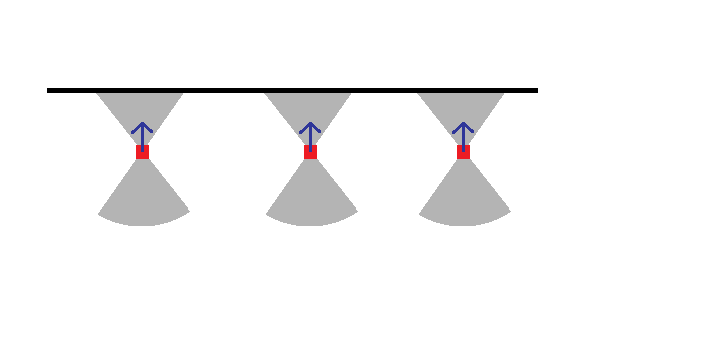
\includegraphics[width=0.9\textwidth]{./images/chapter5/set_one_front.png}
         \label{fig:set_one_front}
     \end{subfigure}%
     \begin{subfigure}[b]{0.5\textwidth}
         \centering
         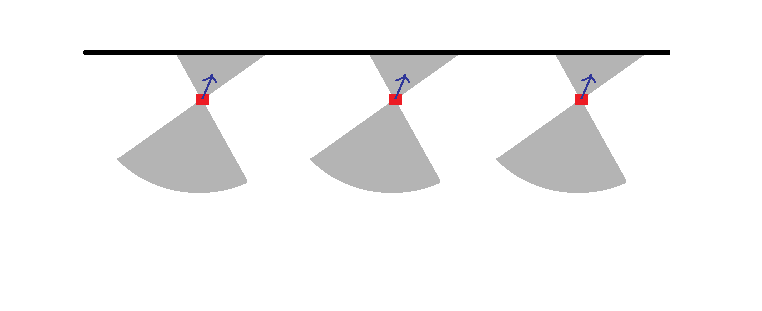
\includegraphics[width=0.9\textwidth]{./images/chapter5/set_two_front.png}
         \label{fig:set_two_front}
     \end{subfigure}
     \hfill
     
     \begin{subfigure}[b]{0.5\textwidth}
         \centering
         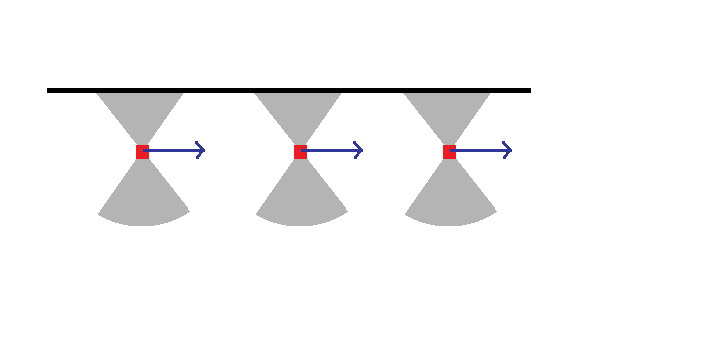
\includegraphics[width=0.9\textwidth]{./images/chapter5/set_one_side.png}
         \label{fig:set_one_side}
     \end{subfigure}%
    %  \hfill
     \begin{subfigure}[b]{0.5\textwidth}
         \centering
         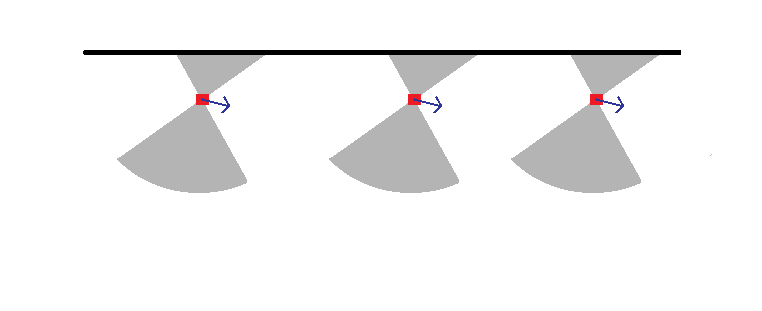
\includegraphics[width=0.9\textwidth]{./images/chapter5/set_two_side.png}
         \label{fig:set_two_side}
     \end{subfigure}
    \caption{Παραδείγματα διαφορετικών προσανατολισμών}
    \label{fig:different_yaw_examples}
\end{figure}


\begin{algorithm}[!htb]
\caption{Find Weights}
\label{alg:find_weights}
\begin{algorithmic}[1]
    \Function{findWeights}{sensor\_number, sensor\_direction, sensor\_fov}
        \State $angles = []$
        \For{$s$ in $range(sensor\_number)$}
            \State $theta = sensor\_direction[s]$
            \State Transform $theta$ to range $[0,90]$
            \State $angles.append((90-theta)/90)$
        \EndFor
        \State $obstacle\_weight = 1 + mean(angles)$
        \State $rotation\_weight = 2 - mean(angles)$
        \State \Return $obstacle\_weight, rotation\_weight$
\end{algorithmic}
\end{algorithm}



\subsection{Προσομοίωση κάλυψης του χώρου και διαγραφή περιττών σημείων}
\label{subsection:node_elimination}

Τελευταίο βήμα της δημιουργίας της πρώτης στρατηγικής πλοήγησης είναι η εκ των προτέρων εκτίμηση της κάλυψης του χώρου και η διαγραφή των στόχων που είναι περιττοί στην όλη διαδικασία. Η εκτίμηση της κάλυψης πραγματοποιείται προσομοιώνοντας τη μέτρηση των αισθητήρων του οχήματος για κάθε στόχο της ακολουθίας. Με τον τρόπο αυτό αποθηκεύονται σε ένα OGM τα σημεία τα οποία πρόκειται να καλυφθούν. Αυτή είναι η απλή περίπτωση με την οποία μπορεί να υπολογιστεί και το ποσοστό κάλυψης των εμποδίων του χώρου, όπως και έγινε στα πειράματα των πινάκων  \ref{tab:motor_schema_weights_side_antennas} και \ref{tab:motor_schema_weights_front_back_antennas}. Σημειώνεται ότι η κάλυψη αυτή είναι μια εκτίμηση, καθώς η πλοήγηση του οχήματος δεν περιλαμβάνεται στο σημείο αυτό με αποτέλεσμα να μην λαμβάνονται υπόψη οι ενδιάμεσες κινήσης μετάβασης από το κάθε σημείο στο επόμενο. Μάλιστα, η τελική πραγματική κάλυψη θα είναι, θεωρητικά, μεγαλύτερη της εκτίμησης.

Ένα παράδειγμα εκτίμησης κάλυψης παρουσιάζεται στο σχήμα \ref{fig:coverage_estimation_ogm_example}, όπου φαίνονται με διάφορες αποχρώσεις του μπλε τους στόχους και με σκούρο γκρι την περιοχή που εκτιμάται ότι θα καλύψει το όχημα από όλα τα σημεία. Επίσης, οπτικοποιείται και η σειρά προσπέλασης, η οποία εκκινεί για κάθε δωμάτιο από τα πιο σκούρα σημεία και κατευθύνεται στα πιο ανοικτόχρωμα, καταλήγοντας στα λευκά.

\begin{figure}[!htb]
    \centering
    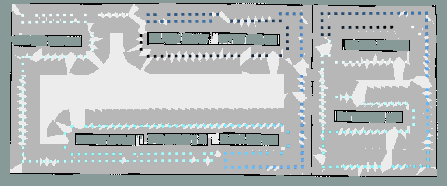
\includegraphics[width=0.9\textwidth]{./images/chapter5/warehouse_4_wall_follow_a_priori_coverage_085_cover_first_weights_2_1_multi_yaw_060.png}
    \caption{Παράδειγμα Πεδίου Εκτίμησης Κάλυψης}
    \label{fig:coverage_estimation_ogm_example}
\end{figure}

Αντίθετα, η διαγραφή σημείων προϋποθέτει τον έλεγχο κάθε φορά των εμποδίων που πρόκειται να καλυφθούν. Εαν το μεγαλύτερο ποσοστό τους είναι ήδη καλυμμένο, τότε το σημείο αυτό είναι περιττό για την μελέτη αυτή. Στόχος είναι να καλυφθεί όσο το δυνατό μεγαλύτερη επιφάνεια εμποδίων, δηλαδή ένα ποσοστό που πλησιάζει το 100\%. Μετά από ορισμένες δοκιμές βρέθηκε ότι το όριο του 85\% προσφέρει καλή συνολική κάλυψη του χώρου. Η χρήση μεγαλύτερων ορίων, όπως τα 90\% και 95\%, οδηγεί σε αποθήκευση πολλών περιττών θέσεων - στόχων χωρίς βελτίωση στην συνολική τελική κάλυψη του χώρου, ενώ το μικρότερο όριο 80\% οδηγεί σε μείωση της κάλυψης. Συνεπώς, για κάθε σημείο υπολογίζονται τα εμπόδια που πρόκειται να σαρώσουν οι αισθητήρες και εφόσον περισσότερο από το 85\% των σημείων είναι ήδη καλυμμένα, τότε ο στόχος αυτός διαγράφεται από την ακολουθία. Τονίζεται ότι τα σημεία εισόδου και εξόδου κάθε χώρου, δηλαδή οι κόμβοι πόρτες, είναι απαραίτητοι για την ομάλη μετάβαση του οχήματος στον χώρο και, επομένως, δεν επιδέχονται διαγραφής.

Ο \ref{alg:check_and_update_cover} υπολογίζει τα σημεία που σαρώνουν οι αισθητήρες για μια δεδομένη πόζα του οχήματος και στη συνέχεια υπολογίζει πόσα από αυτά έχουν ήδη σαρωθεί. Εαν το ποσοστό είναι μεγαλύτερο από το $threshold$ τότε η πόζα αυτή απορρίπτεται, ειδάλλως προστίθεται κανονικά στην τελική ακολουθία.

Ο \ref{alg:a_priori_coverage} αποτελεί τον συγκεντρωτικό αλγόριθμο εκτέλεσης της εκ των προτέρων κάλυψης του χώρου. Ο αλγόριθμος δέχεται ως είσοδο και μια λογική μεταβλητή, την $eliminate$, η οποία καθορίζει εαν θα πραγματοποιηθεί εξάλειψη των περιττών σημείων. Αν αυτή είναι Ψευδής τότε η διαδικασία αποτελεί την απλή εκτίμηση κάλυψης του χώρου, το τελικό OGM της οποίας χρησιμοποιείται για να υπολογιστεί το ποσοστό κάλυψης. Αντίθετα, εαν είναι Αληθής, τότε στόχος είναι η μείωση του μεγέθους της ακολουθίας. Επιπλέον, η εντολή ελέγχου στην όγδοη σειρά είναι αυτή που καθορίζει ποια από τις δύο περιπτώσεις θα κληθεί. Στην εντολή αυτή φαίνεται και το γεγονός ότι ο πρώτος και ο τελευταίος στόχος κάθε δωματίου κρατείται στην τελική ακολουθία για τους λόγους που σχολιάστηκαν νωρίτερα. Τέλος, η διαδικασία πραγματοποιείται για κάθε δωμάτιο και τελικά επιστρέφεται η τελική ακολουθία του πρώτου πρότυπου πλοήγησης.

Στο σχήμα \ref{fig:coverage_estimation_ogm_example} παρουσιάστηκε η περίπτωση η απλή περίπτωση εκτίμησης κάλυψης. Στο \ref{fig:coverage_estimation_ogm_with_elimination_example} παρουσιάζεται η δεύτερη περίπτωση, όπου όσοι στόχοι είναι περιττοί έχουν διαγραφεί. Επίσης, η δειγματοληψία σ αυτό το παράδειγμα έχει πολλά διαφορετικά βήματα, ενώ οι αισθητήρες έχουν μεγαλύτερη ακτίνα λήψης. Τέλος, η μαύρη περιοχή αποτελεί την εκτίμηση της περιοχής που θα σαρωθεί από τους αισθητήρες.


\begin{figure}[!htb]
    \centering
    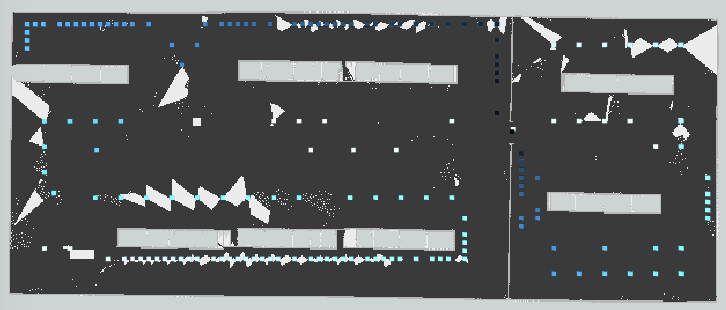
\includegraphics[width=0.9\textwidth]{./images/chapter5/warehouse_4_wall_follow_sampling_without_inloop_elim.png}
    \caption{Παράδειγμα Πεδίου Εκτίμησης Κάλυψης με Διαγραφή Περιττών Σημείων}
    \label{fig:coverage_estimation_ogm_with_elimination_example}
\end{figure}



\begin{algorithm}[H]
\caption{A Priori Coverage}
\label{alg:a_priori_coverage}
\begin{algorithmic}[1]
    \Function{aPrioriCoverage}{ogm, brushfire, nodes, eliminate, resolution, sensor\_range, sensor\_fov, sensor\_direction}
    \State $coverage = numpy.zeros(ogm.shape)$
    \State $new\_nodes = []$
    \For{$room$ in $nodes$}
        \State $new\_room = []$
        \For{$i$ in $range(len(room))$}
            \State $x, y = room[i]['position']$, $yaw = room[i]['yaw']$
            \If{not $i$ or $i == len(room)-1$ or not $eliminate$}
                \State $coverage$, $previous\_robot\_pose =  updateCover($ \par
                \hskip \algorithmicindent $room[i-1]['position'], ogm, coverage, resolution, sensor\_range, $ \par
                \hskip \algorithmicindent $sensor\_fov, sensor\_direction)$
                \State $updated = $True
            \Else
                \State $updated$, $coverage = checkAndUpdateCover(brushire, 0.85, ogm, coverage,$\par 
                \hskip\algorithmicindent $ resolution, sensor\_range, sensor\_fov, sensor\_direction)$
            \EndIf
            \If{$updated$}
                \State $new\_room.append(room[i])$
            \EndIf
        \EndFor
        \State $new\_nodes.append(new\_room)$
        \State $i++$
    \EndFor
    \State \Return $new\_nodes$
\end{algorithmic}
\end{algorithm}



\begin{algorithm}[H]
\caption{Check And Update Cover}
\label{alg:check_and_update_cover}
\begin{algorithmic}[1]
    \Function{checkAndUpdateCover}{brushfire, threshold, ogm, coverage, resolution,  sensor\_range, sensor\_fov, sensor\_direction}
    \State Read robot's pose $xx$, $yy$, $th$
    \State $indexes = []$
    \For{each sensor $s$}
        \State $cover\_length = int(sensor\_range[s] / resolution)$
        \State $temp = circularRayCastCoverage((xx,yy), ogm, cover\_length, sensor\_fov[s],$\par
        \hskip\algorithmicindent $th, sensor\_direction[s])$
        \State $indexes.extend(temp)$
    \EndFor
    \State Compute percentage $perc$ of already covered points of $indexes$
    \State $updated = $False
    \If{$perc < threshold$}
        \State $updated = $True
        \For{$x$, $y$ in $indexes$}
            \State $coverage[x, y] = 100$
        \EndFor
    \EndIf
    \State \Return $updated$, $coverage$
\end{algorithmic}
\end{algorithm}

\subsection{Δημιουργία Αλληλουχίας Κόμβων Ζιγκ-Ζαγκ}
\label{subsection:zig_zag_sequence_implementation}

Το τελευταίο μέρος της υλοποίησης του συστήματος περιέχει την δημιουργία της δεύτερης στρατηγικής πλοήγησης στον χώρο. Αυτή είναι η πλοήγηση με κινήσεις σε μορφή ζιγκ ζαγκ. Η κίνηση του οχήματος χρησιμοποιώντας αυτή την στρατηγική έχει δύο πλεονεκτήματα. Πρώτον, κάθε εμπόδιο θα σαρώνεται περισσότερες φορές και, δεύτερον, οι σαρώσεις θα πραγματοποιούνται με διαφορετικές γωνίες μεταξύ αισθήρα και εμποδίου, προσφέροντας πιο αναλυτική και ομοιόμορφη κάλυψη. Στην ιδανική περίπτωση στόχος είναι να σαρωθεί ένα εμπόδιο τόσο από το θετικό μισό τόξο του αισθητήρα, όσο και από το αρνητικό \ref{fig:different_angle_cover_example}. Βέβαια, όσες περισσότερες φορές και υπό διαφορετικές γωνίες σαρώσουν οι αισθητήρες ένα σημείο, τόσο πιο βέβαιο θα είναι το αποτέλεσμα. Το σημαντικό μειονέκτημα, όμως, της περίπτωσης αυτής είναι η αύξηση του συνόλου των στόχων που έχει να προσεγγίσει το όχημα και, επομένως, η αύξηση του συνολικού χρόνου κάλυψης του χώρου.

Ένας πολύ απλός και ταυτόχρονα αποτελεσματικός τρόπος παραγωγής μιας τέτοιας πορείας είναι η προσθήκη σημείων στόχων στην ήδη υπάρχουσα βέλτιστη ακολουθία, με στόχο την δημιουργία ζιγκ ζαγκ κινήσεων. Η προσθήκη τέτοιων στόχων μεταξύ των συνεχώμενων γειτονικών σημείων με μια μικρή απόκλιση από την μεταξύ τους ευθεία θα επιφέρει το επιθυμητό αποτέλεσμα. Ο αλγόριθμος αυτός παρουσιάζεται στο \ref{alg:add_zig_zag_nodes} και αναλύεται στη συνέχεια. Η ακολουθία κάθε δωματίου εξετάζεται χωριστά. Τα ήδη υπολογισμένα σημεία διατηρούνται ανέπαφα και ενδιάμεσα τους προστίθενται νέα, όπου κρίνεται απαραίτητο. Η διαδικασία εκμεταλλεύεται το γεγονός ότι η δειγματοληψία που έχει υλοποιηθεί έχει σταθερά βήματα, συνεπώς είναι εύκολα διακριτό εαν δύο σημεία βρίσκονται πολύ κοντά και χρίζουν προσθήκης νέων ενδιάμεσων στόχων. Θα έχουν μια από τις δύο μεταβλητές θέσης ίσες, πράγμα δεδομένο λόγω της ομοιόμορφης δειγματοληψίας σε κάθε βήμα. Εαν ισχύει αυτό και τα δύο σημεία είναι αρκετά κοντά, αλλά δεν ταυτίζονται, τότε προστίθεται ένας ακόμη στόχος. Υπολογίζεται η μέση των δύο σημείων και η απόσταση του νέου σημείου από την ευθεία τους η οποία είναι η μισή από την μεταξύ τους απόσταση, ώστε η τροχιά του οχήματος να είναι όσο πιο ομαλή γίνεται. Από τις δύο υποψήφιες θέσεις επιλέγεται αυτή με μεγαλύτερη τιμή brushfire, καθώς θα απέχει μεγαλύτερη απόσταση από τα εμπόδια. Έπειτα, καθώς κάθε στόχος περιέχει και τον προσανατολισμό του οχήματος, τίθεται ως τιμή στροφής του οχήματος η γωνία της ευθείας μεταξύ του τρέχοντος σημείου και του νέου, κάτι που δεν θα επηρεάζει, δηλαδή, τη συνολική κίνηση του οχήματος. Τέλος προκειμένου, να προστεθεί στην αλληλουχία το νέο σημείο πρέπει να ανήκει στο εν λόγω δωμάτιο, γι αυτό και πραγματοποιείται ο αντίστοιχος έλεγχος. 

Η διαδικασία οπτικοποιείται στο \ref{fig:example_zig_zag_choice}. Τα κόκκινα σημεία έχουν βρεθεί μέσω της δειγματοληψίας και είναι πολύ κοντά, συνεπώς μπορεί να προστεθεί ένας ακόμη στόχος ενδιάμεσα τους για να προκληθεί η ζιγκ ζαγκ κίνηση. Η ευθεία των σημείων σημειώνεται με πράσινο. Τα μπλε σημεία είναι τα δύο υποψήφια να προστεθούν στην ακολουθία, τα οποία βρίσκονται πάνω στην μεσοκάθετο του ευθύγραμμου τμήματος των δύο σημείων. Επιλέγεται, τελικά, αυτό που απέχει την μεγαλύτερη απόσταση από τα γύρω εμπόδια, δηλαδή το κάτω σημείο, το οποίο και έχει κυκλωθεί. Ένα παράδειγμα ζιγκ ζαγκ κίνησης μπροστά από ένα εμπόδιο είναι το \ref{fig:example_zig_zag_path}.


\begin{figure}[!htb]
    \centering
    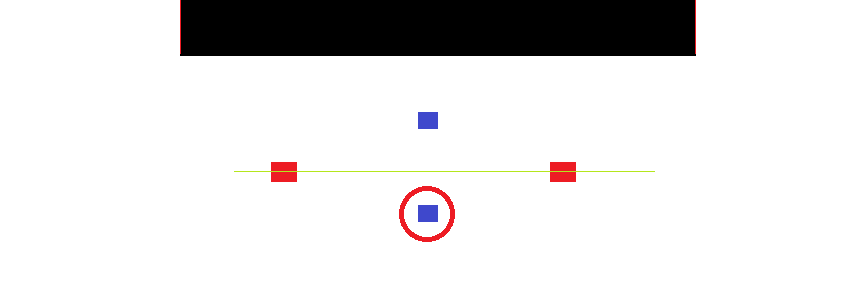
\includegraphics[width=0.8\textwidth]{./images/chapter5/example_zig_zag_choice.png}
    \caption{Παράδειγμα Επιλογής Ζιγκ Ζαγκ Σημείου}
    \label{fig:example_zig_zag_choice}
\end{figure}




\begin{figure}[!htb]
    \centering
    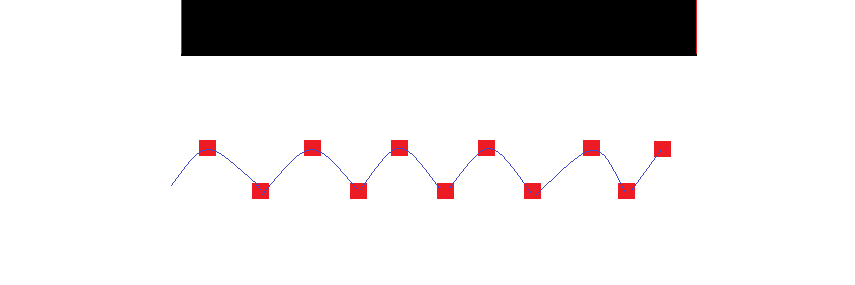
\includegraphics[width=0.8\textwidth]{./images/chapter5/example_zig_zag_path.png}
    \caption{Παράδειγμα Κίνησης Ζιγκ Ζαγκ παράλληλα με ένα εμπόδιο}
    \label{fig:example_zig_zag_path}
\end{figure}


\begin{algorithm}[H]
\caption{Add Zig Zag Nodes}
\label{alg:add_zig_zag_nodes}
\begin{algorithmic}[1]
    \Function{addZigZagNodes}{sequence, brushfire, ogm, sensor\_range, resolution}
        \State $zig\_zag\_sequence = []$
        \For{each $room$ in $sequence$}
            \State $temp\_sequence = []$
            \For{$i$ in $range(len(room))$}
                \If{not $i$}
                    \State $temp\_sequence.append(room[i])$
                    \State continue
                \EndIf
                \State $node = room[i]['position']$, $previous\_node = room[i-1]['position']$
                \State $x\_final, y\_final = 0, 0$
                \If{$previous\_node[0] == node[0]$ and $abs(previous\_node[1]-node[1])$ and $abs(previous\_node[1]-node[1]) <= max(sensor\_range)/ resolution$}
                    \State $dif = abs(previous\_node[1]-node[1])$
                    \State $x1 = int(node[0] - dif/2)$, $x2 = int(node[0] + dif/2)$
                    \State $y = int(min([previous\_node[1],node[1]]) + dif/2)$
                    \If{$brushfire[x1,y] >= brushfire[x2,y]$}
                        \State $x\_final = x1$, $y\_final = y$, $yaw = math.degrees(math.atan2(y-node[1], x1-node[0]))$
                    \Else
                         \State $x\_final = x2$, $y\_final = y$, $yaw = math.degrees(math.atan2(y-node[1], x2-node[0]))$
                    \EndIf
                \ElsIf{$previous\_node[1] == node[1]$ and $abs(previous\_node[0]-node[0])$ and $abs(previous\_node[0]-node[0]) <= max(sensor\_range)/resolution$}
                    \State $dif = abs(previous\_node[0]-node[0])$
                    \State $y1 = int(node[1] - dif/2)$, $y2 = int(node[1] + dif/2)$
                    \State $y = int(min([previous\_node[0],node[0]]) + dif/2)$
                    \If{$brushfire[x,y1] >= brushfire[x,y2]$}
                        \State $x\_final = x$, $y\_final = y1$, $yaw = math.degrees(math.atan2(y1-node[1], x-node[0]))$
                    \Else
                         \State $x\_final = x$, $y\_final = y2$, $yaw = math.degrees(math.atan2(y2-node[1], x-node[0]))$
                    \EndIf
                \EndIf
                \If{$(x\_final,y\_final)$ is point of $room$}
                    \State $temp\_sequence.append({'position': (x\_final,y\_final), 'yaw': yaw})$
                \EndIf
                \State $temp\_sequence.append(room[i])$
            \EndFor
            \State $zig\_zag\_sequence.append(temp\_sequence)$
        \EndFor
        \State \Return $zig\_zag\_sequence$
\end{algorithmic}
\end{algorithm}


